\documentclass[8pt]{beamer}



\mode<presentation>
{
%  \usetheme{Berkeley}
	\usetheme{Dresden}
%	\usetheme{Berlin}
%   \usecolortheme{dove}
%   \usecolortheme{dolphin}
%   \useinnertheme{circles}
   
  \setbeamercovered{transparent}

}


\usepackage[english]{babel}
\usepackage[utf8]{inputenc}
\usepackage{times}
\usepackage[T1]{fontenc}
\usepackage{multimedia}
\usepackage[absolute,overlay]{textpos}
\usepackage{graphicx}

\usepackage{xcolor}
\usepackage{amsmath}
\usepackage[absolute,overlay]{textpos}
\usepackage{physics}
\usepackage{fixltx2e}

\graphicspath{{./media/images/}}

\definecolor{paint}{RGB}{150,0,0}
\setbeamercolor {structure} {fg=paint}
%\setbeamercolor{title}{fg=black}
%\setbeamertemplate{itemize items}[circle]




\newcommand{\jsqrt}[2]{\bqty{ #1 #1 | #2 #2 }}
\newcommand{\ksqrt}[2]{\bqty{ #1 #2 | #2 #1 }}
\newcommand\mf[1]{\mathbf{#1}}
\newcommand\dens{\rho(\mathbf{r})}
\newcommand\densin{\rho^{in}(\mathbf{r})}
\newcommand\densout{\rho^{out}(\mathbf{r})}
\newcommand\rdens{\tilde{\rho}(\mathbf{G})}
\newcommand\erre{\mathbf{r}}
\newcommand\GI{\mathbf{G}}
\newcommand\QE{\textsc{Quantum} ESPRESSO }
\newcommand\numbands{n_{bands}}
\newcommand\numG{n_{G}}
\newcommand\numR{n_{R}}
\newcommand\bigO{\mathcal{O}}
\newcommand\CO{Co\textsubscript{3}O\textsubscript{4} } 


\title[Tuning the computational architecture for Quantum Espresso \textit{ab initio} calculation of nanostructures] % (optional, use only with long paper titles)
{Tuning the computational architecture for Quantum Espresso \textit{ab initio} calculation of nanostructures}

\author[Giorgio Ruffa] 
{Giorgio Ruffa}
\institute[Università degli Studi di Milano]{Università degli Studi di Milano}

\date{28 Aprile 2016} 

\subject{}


\begin{document}

% ********** 1 slide *****************
\begin{frame}
  \titlepage
\end{frame}

\section{Introduzione}
\subsection{Density Functional Theory}
% ********** slide 2 *****************

\begin{frame}{Introduzione}
\begin{center}
		
\includegraphics[width=4cm]{beam_qe_logo.jpg}
\end{center}
\begin{columns}
	\column{0.33\textwidth}
		\begin{center}
			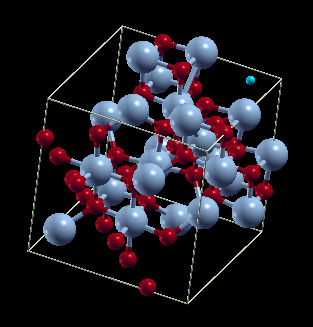
\includegraphics[height=3.5cm]{beam_co3.png}
		\end{center}
	\column{0.33\textwidth}
		\begin{center}
			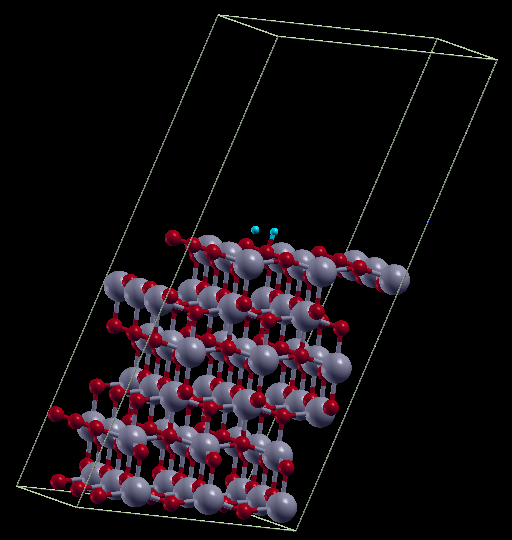
\includegraphics[height=3.5cm]{titania_crystal.png}
		\end{center}
	\column{0.33\textwidth}
		\begin{center}
			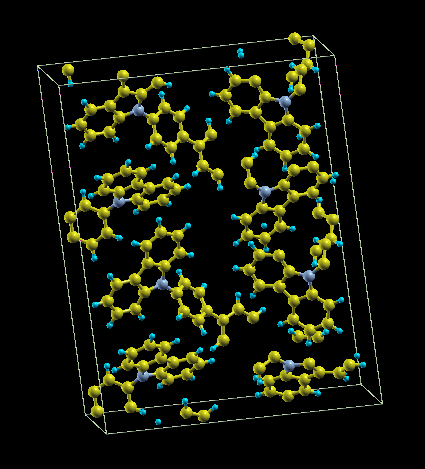
\includegraphics[height=3.5cm]{beam_cbp.png}
		\end{center}
\end{columns}
		
\end{frame}

% ********** slide 3 *****************
\begin{frame}{Introduzione}


\begin{columns}
	\column{0.5\textwidth}
%		\begin{center}
%			
\includegraphics[width=4cm]{beam_qe_logo.jpg}		
%		\end{center}
	
	\invisible<1>{\begin{block}{Density Functional Theory (DFT)}
		\begin{itemize}
			\setlength\itemsep{1em}
			\item[]<2-> Equazioni di Kohn-Sham :
			\item[]<2-> $ \displaystyle  \lbrace  - \frac{1}{2} \nabla^2+ v_{eff}(\erre) \rbrace 	\psi_{j}^{KS}(\erre) = \varepsilon_{j}^{KS} 	\psi_{j}^{KS}(\erre)$
			\item[]<3-> $ \displaystyle  v_{eff}(\erre) = v_{ion}(\erre) + v_{h}(\erre) + v_{xc}(\erre)$
			\item[]<3-> $ \displaystyle v_{h}(\erre) = \int \frac{\rho(\erre')}{\mid \erre - \erre'\mid} \dd{\erre'} $
			\item[]<3-> $ \displaystyle v_{xc}(\erre) =	\frac{\var{E_{xc}[\dens]}}{\var{\dens}}$
		\end{itemize}
	\end{block}}
		
	\column{0.5\textwidth}
		\begin{center}

			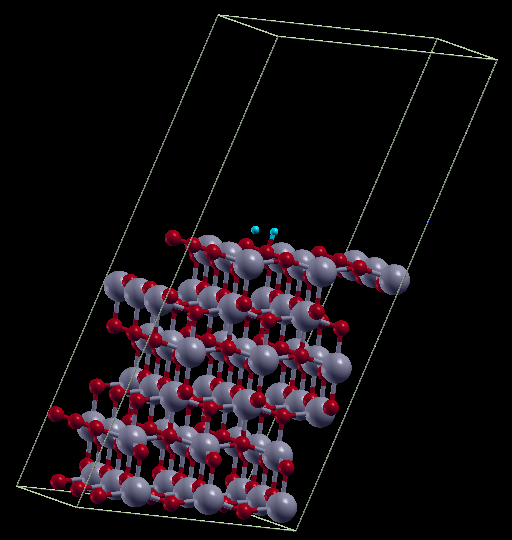
\includegraphics[width=3.5cm]{titania_crystal.png}	\\

			~ \\
			Superficie TiO\textsubscript{2} : \\ $ 150$ Atomi $\sim 2 \cdot 10 ^{3} e^{-}$	

		\end{center}
\end{columns}

\end{frame}

% ********** slide 4 *****************
\begin{frame}{Self Consistent DFT}
\begin{center}
	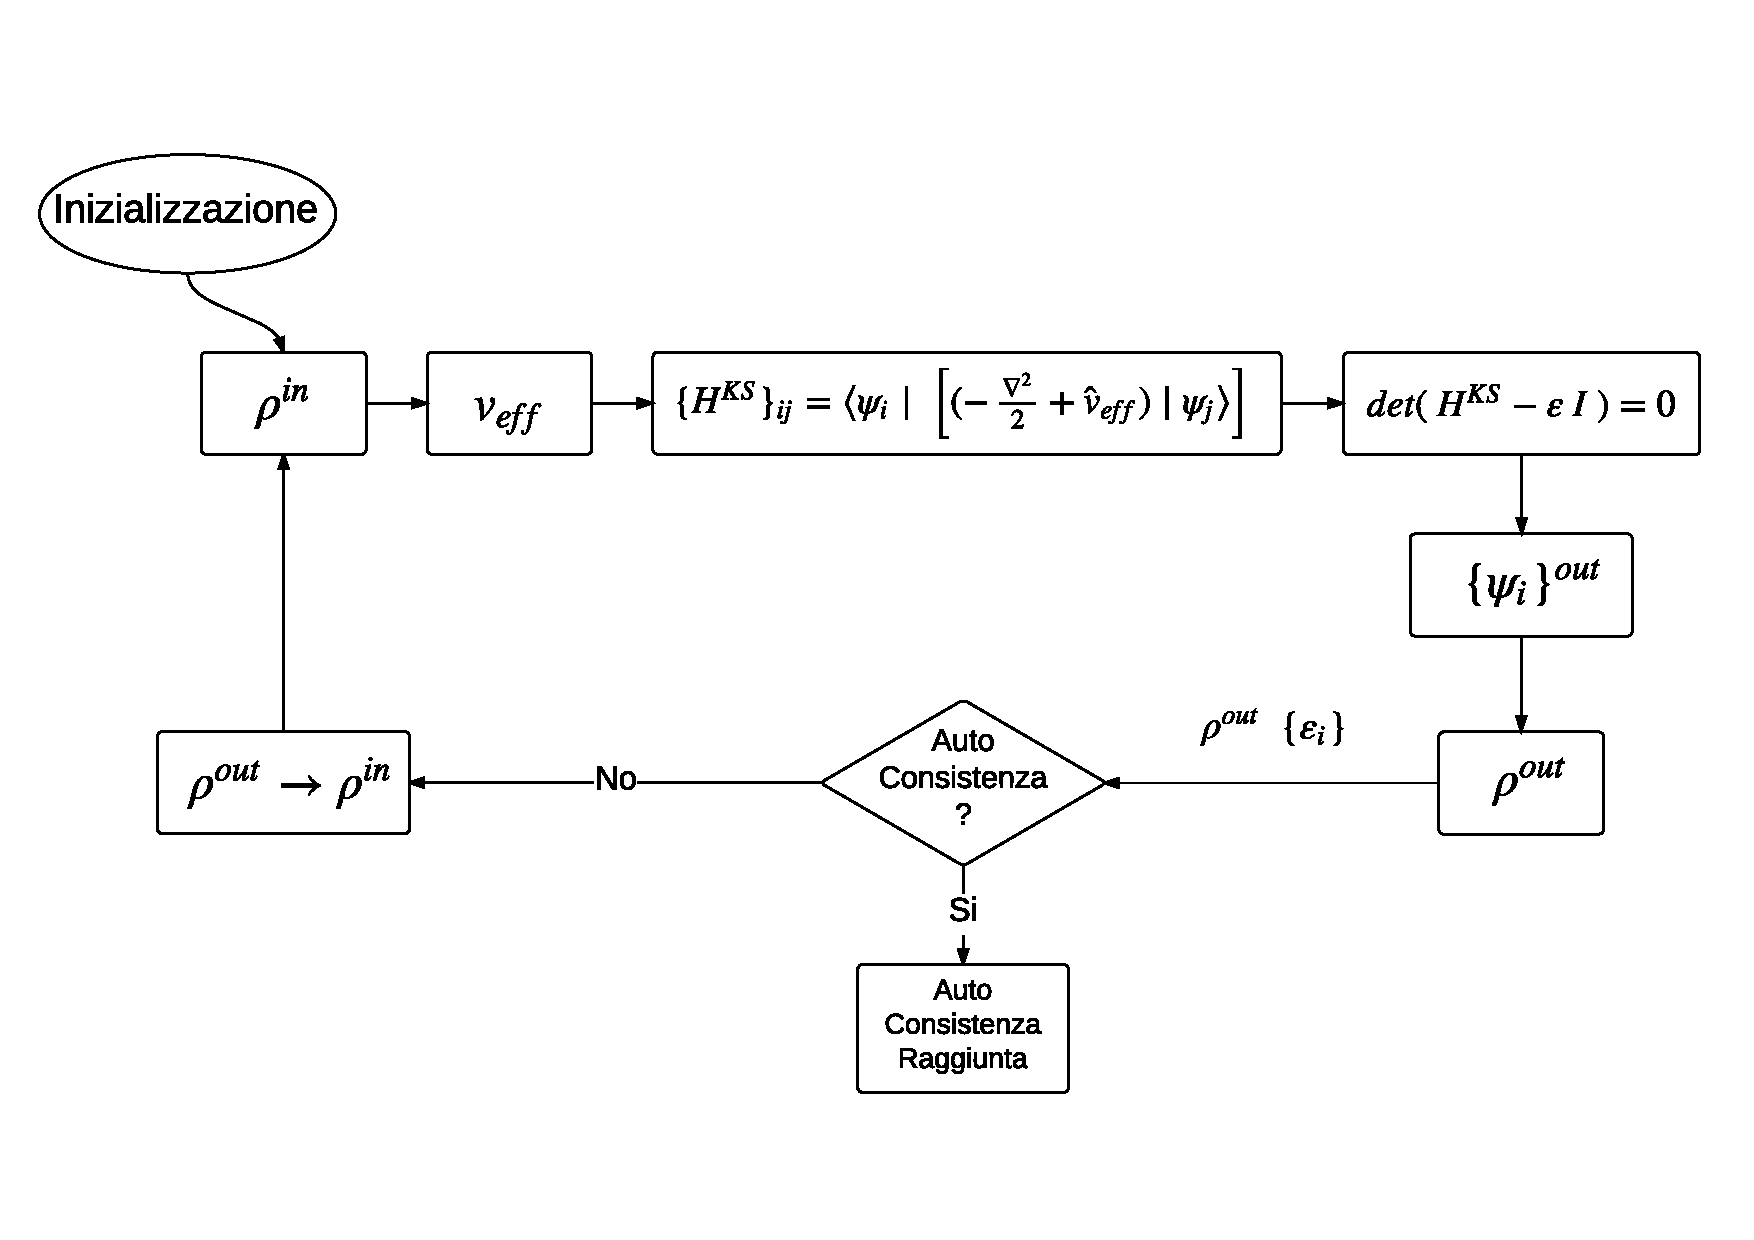
\includegraphics[width=\textwidth]{beam_SCF_0.pdf}	
\end{center}
\end{frame}


% ********** slide 5 *****************}

\def \inputPos {3}
\def \electronsPos {4}
\def \cegtergPos {5}
\def \hpsiPos {6}
\def \cdiaghgPos {7}
\def \sumbandPos {8}
\def \fftPos {9}
\def \fftscatterPos {10}
\def \scfPicWidth {1.1}
\def \scfPicHeight {0.62}

\begin{frame}{Funzioni rilevanti}
\vbox{
    \begin{minipage}[t][0.5\textheight][t]{\textwidth}
    	\begin{columns}
    		\column{0.5\textwidth}

			   \begin{flushleft}
			   	\only<1,\fftPos,\fftscatterPos>{
					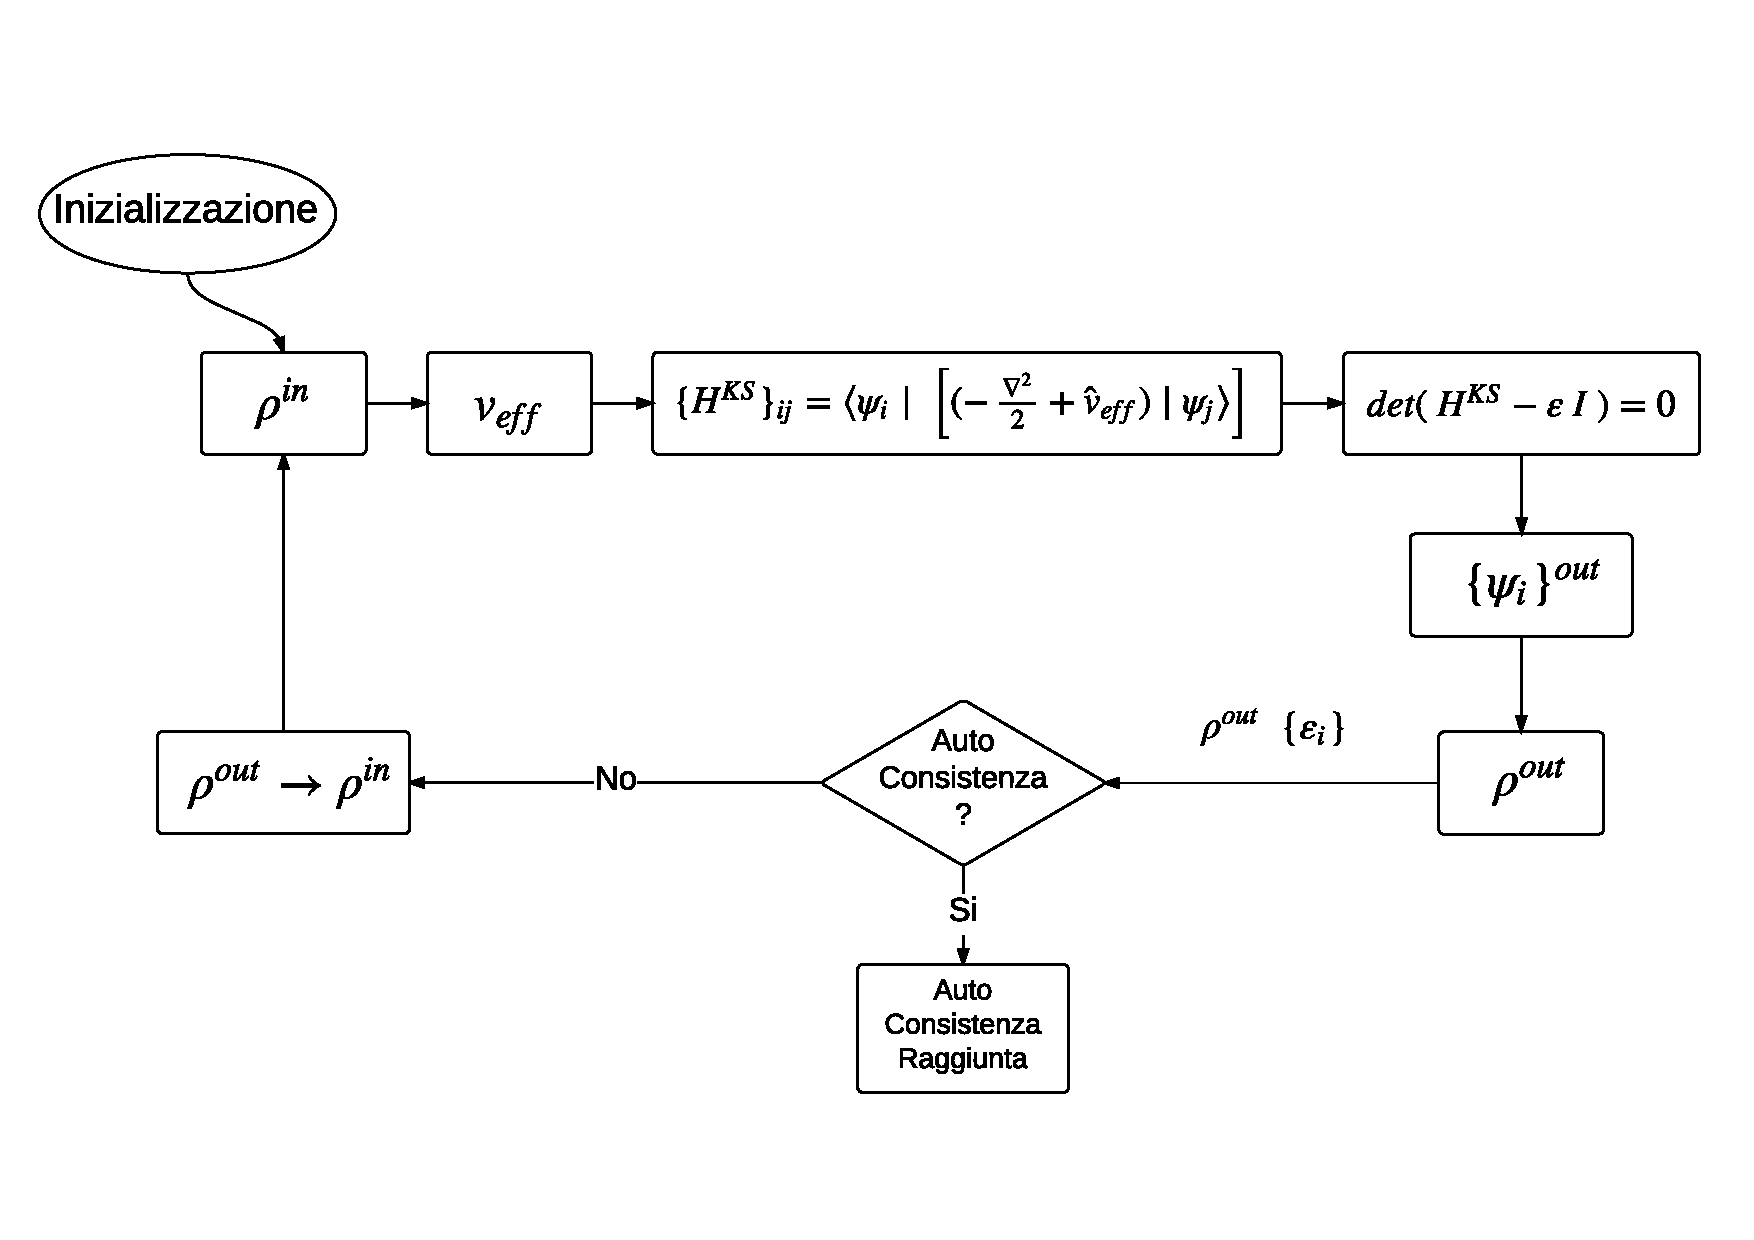
\includegraphics[height=\scfPicHeight\textheight, width=\scfPicWidth\textwidth]{beam_SCF_0.pdf}	
				}
				\only<2>{
					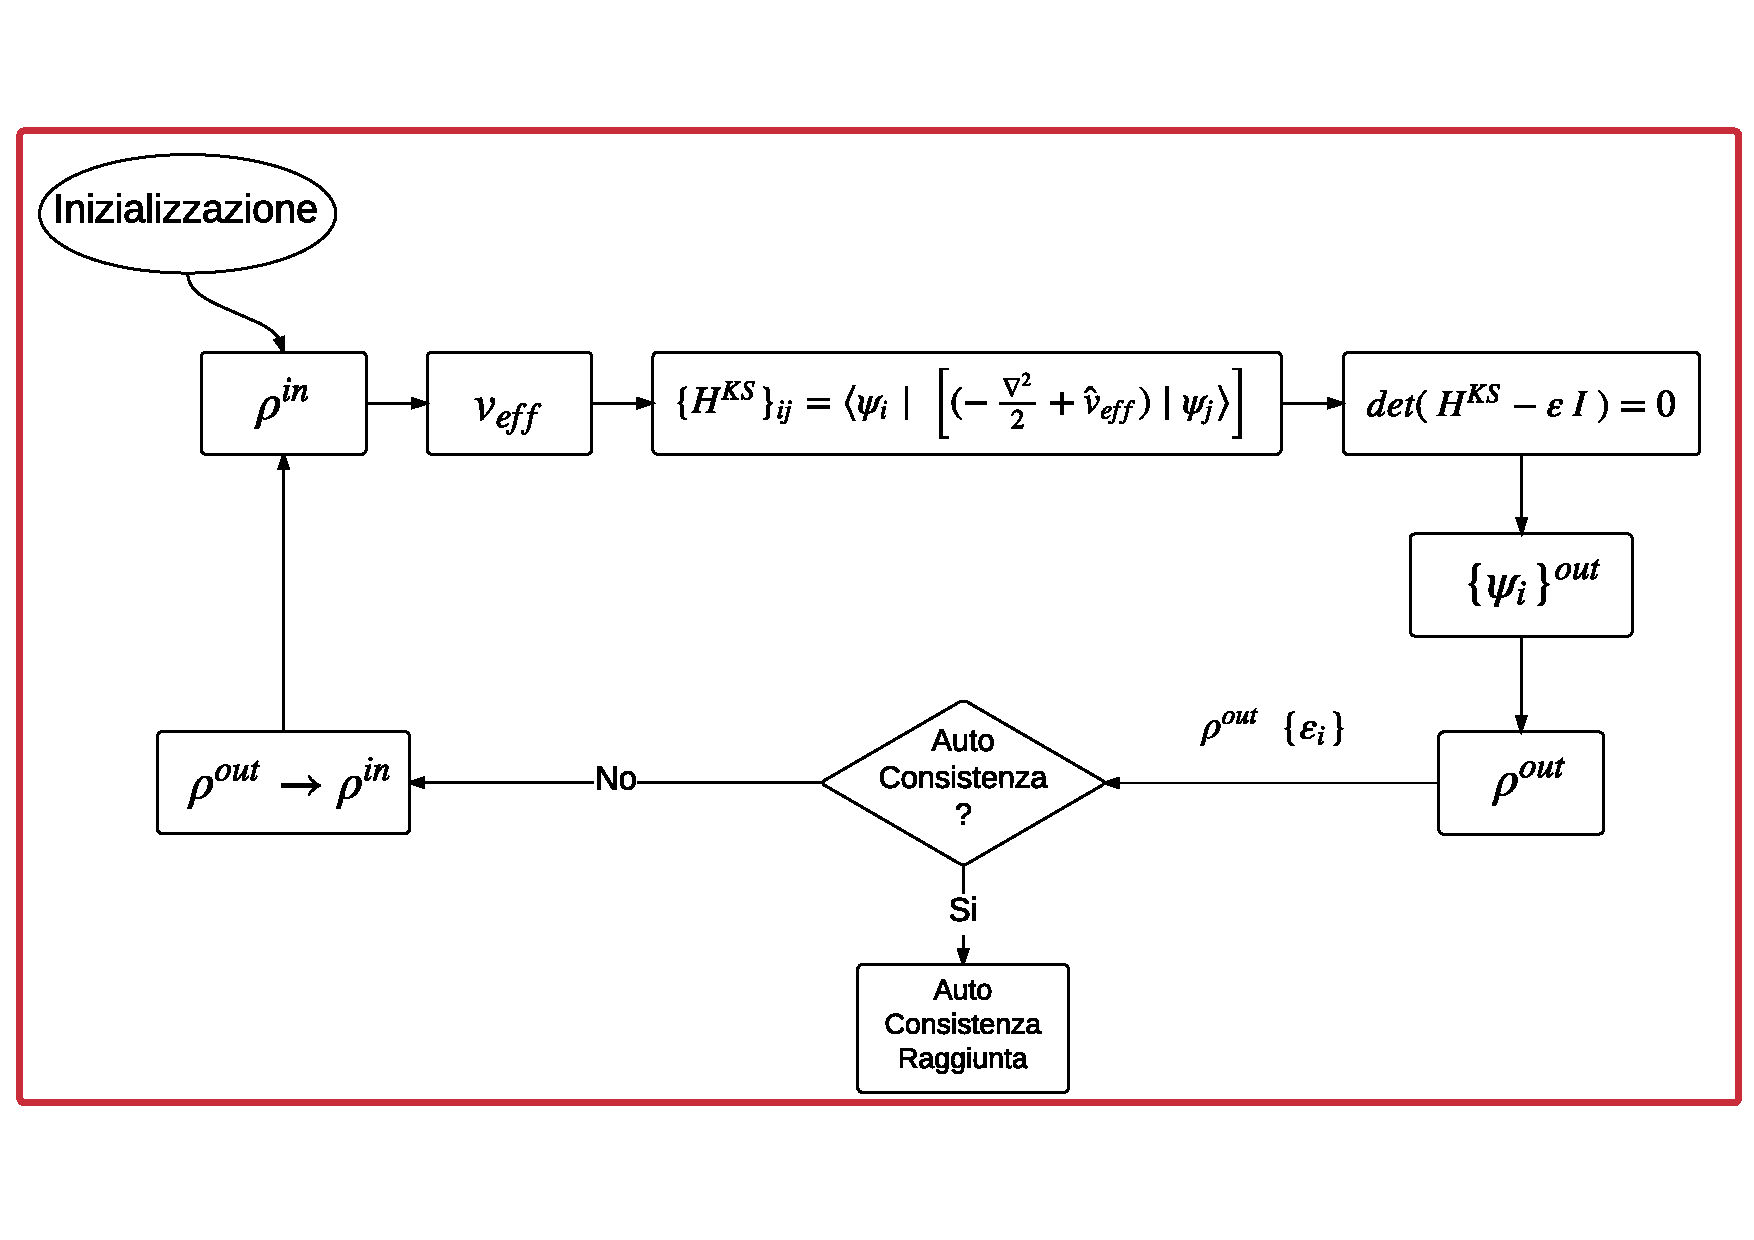
\includegraphics[height=\scfPicHeight\textheight, width=\scfPicWidth\textwidth]{beam_SCF_PWSCF.pdf}	
				}
				\only<\inputPos>{
					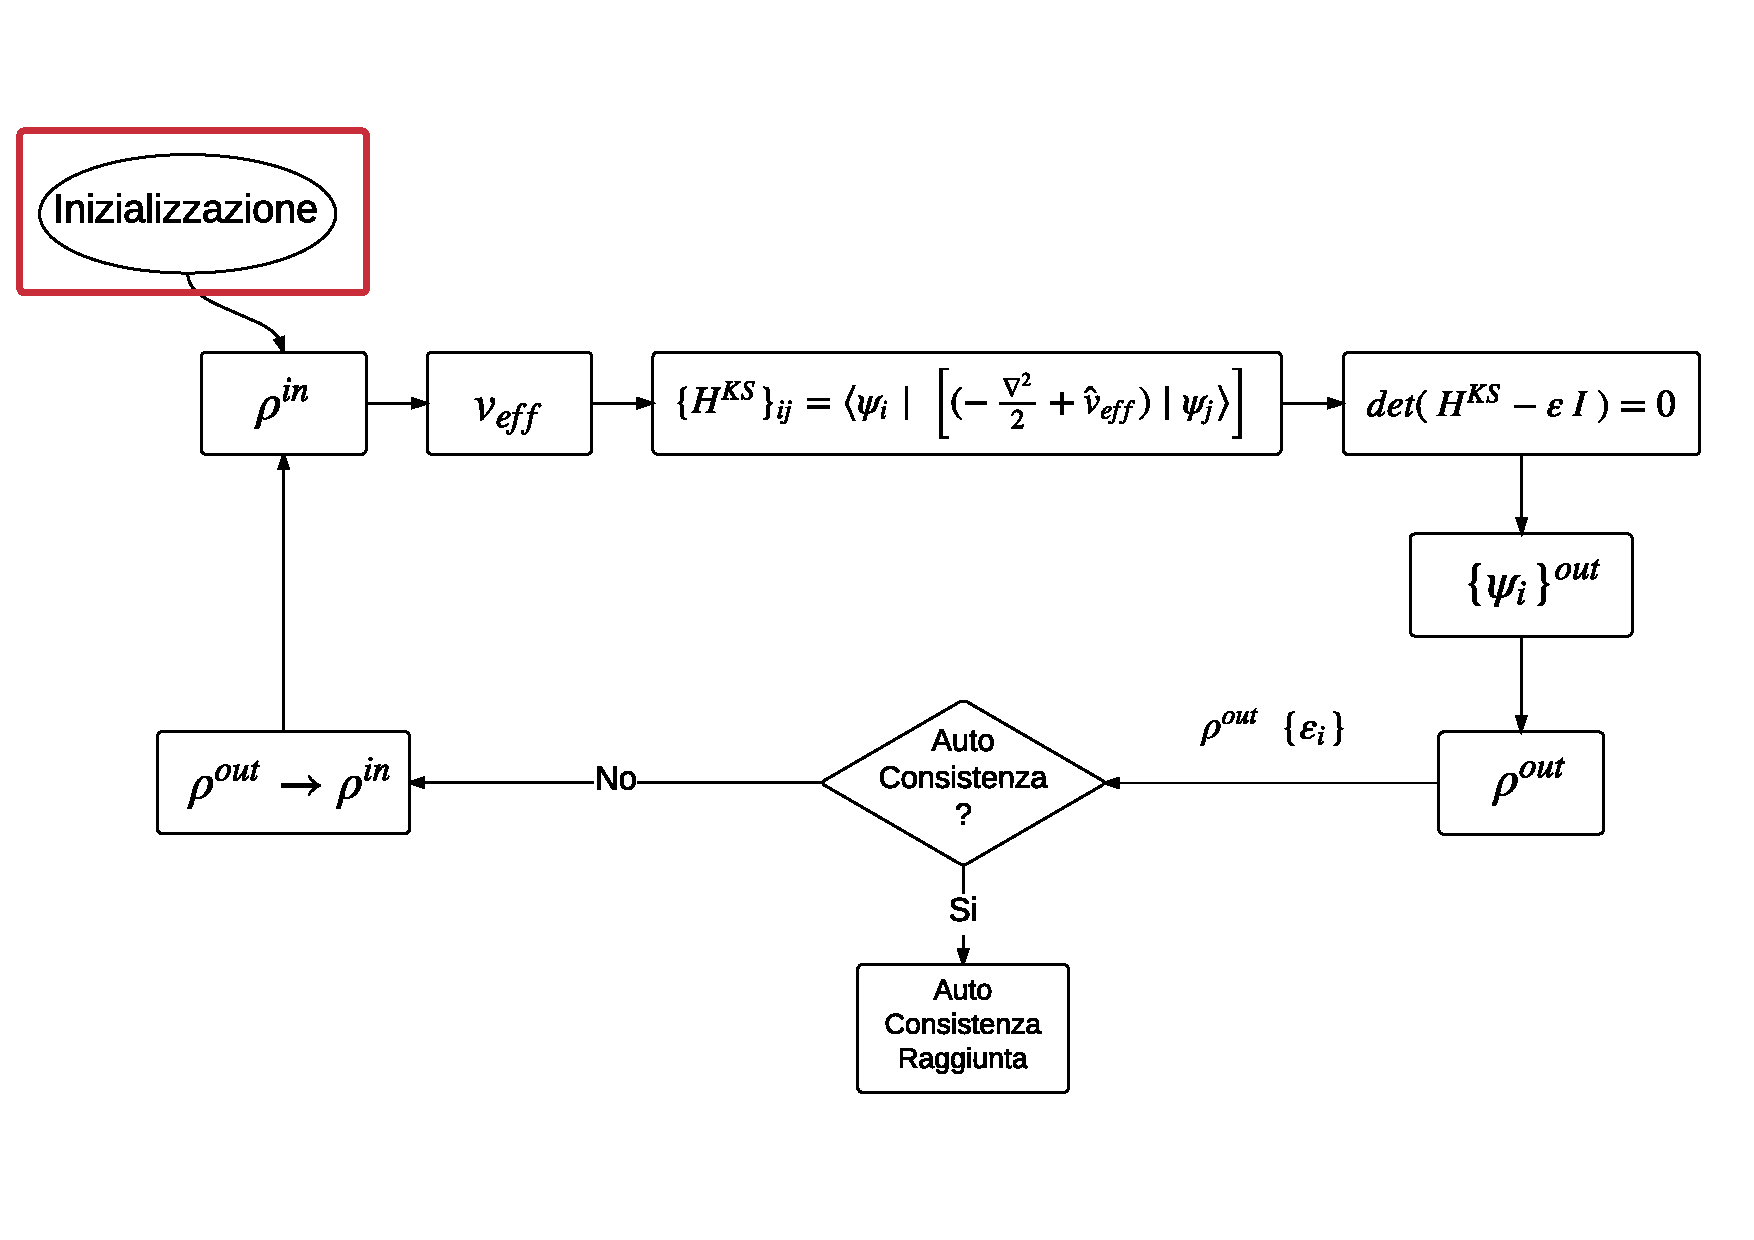
\includegraphics[height=\scfPicHeight\textheight, width=\scfPicWidth\textwidth]{beam_SCF_init_run.pdf}	
				}
				\only<\electronsPos>{
					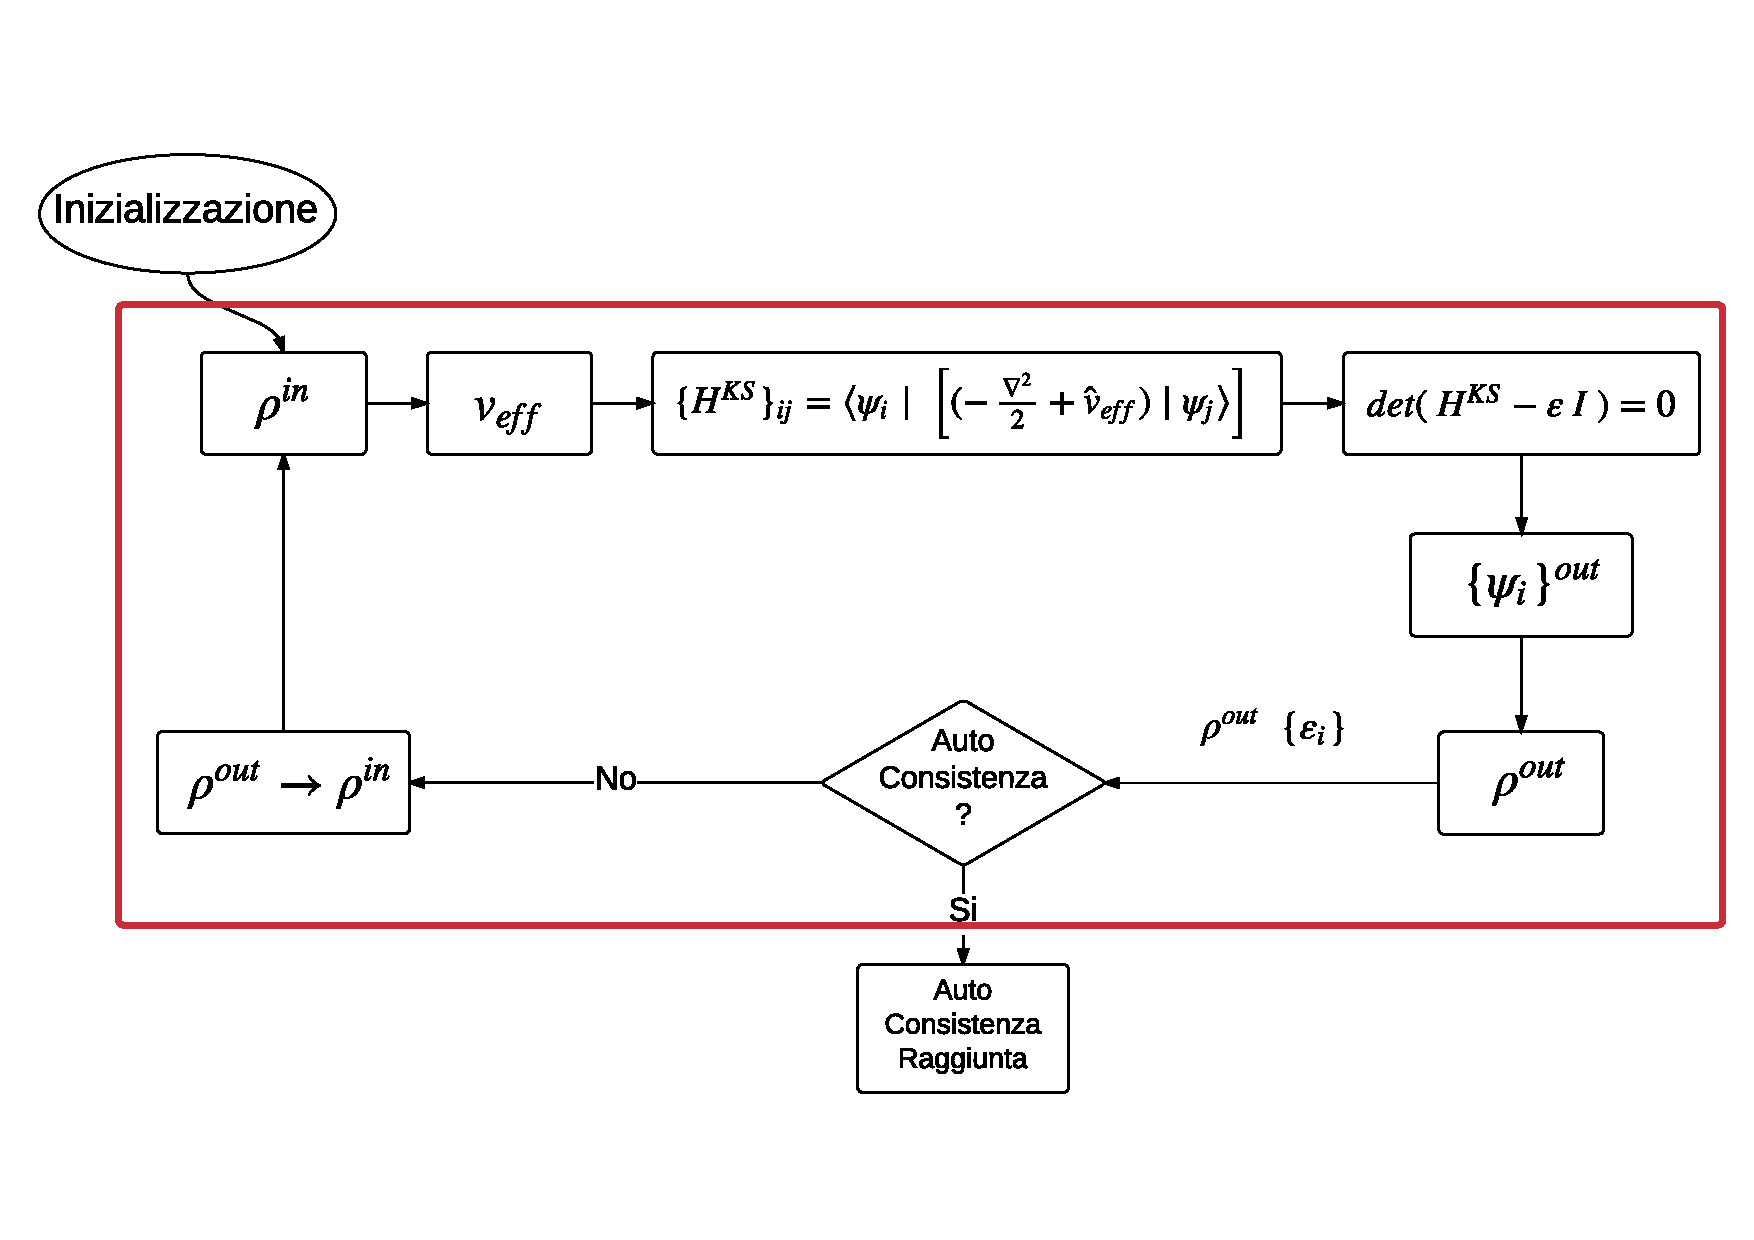
\includegraphics[height=\scfPicHeight\textheight, width=\scfPicWidth\textwidth]{beam_SCF_electrons.pdf}	
				}				
				\only<\cegtergPos>{
					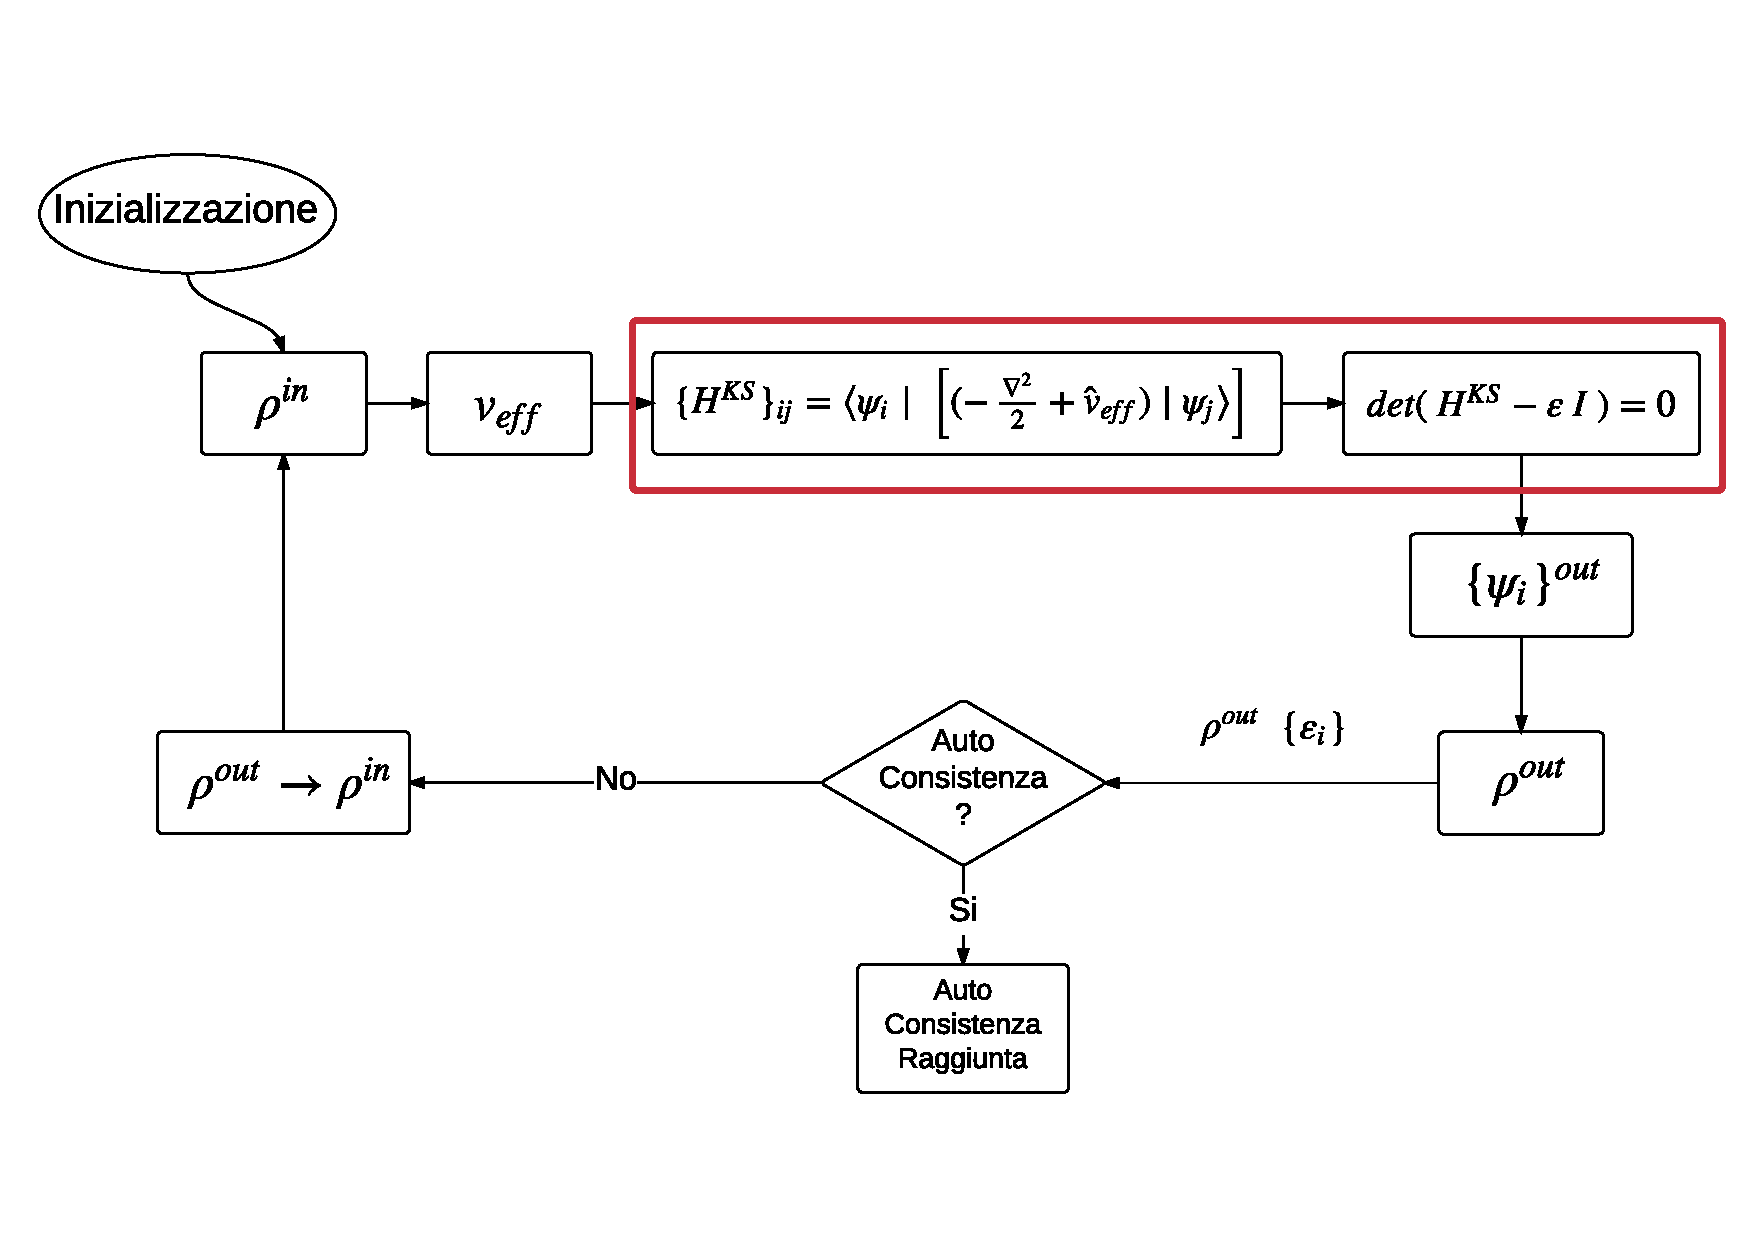
\includegraphics[height=\scfPicHeight\textheight, width=\scfPicWidth\textwidth]{beam_SCF_cegterg.pdf}	
				}
				\only<\hpsiPos>{
					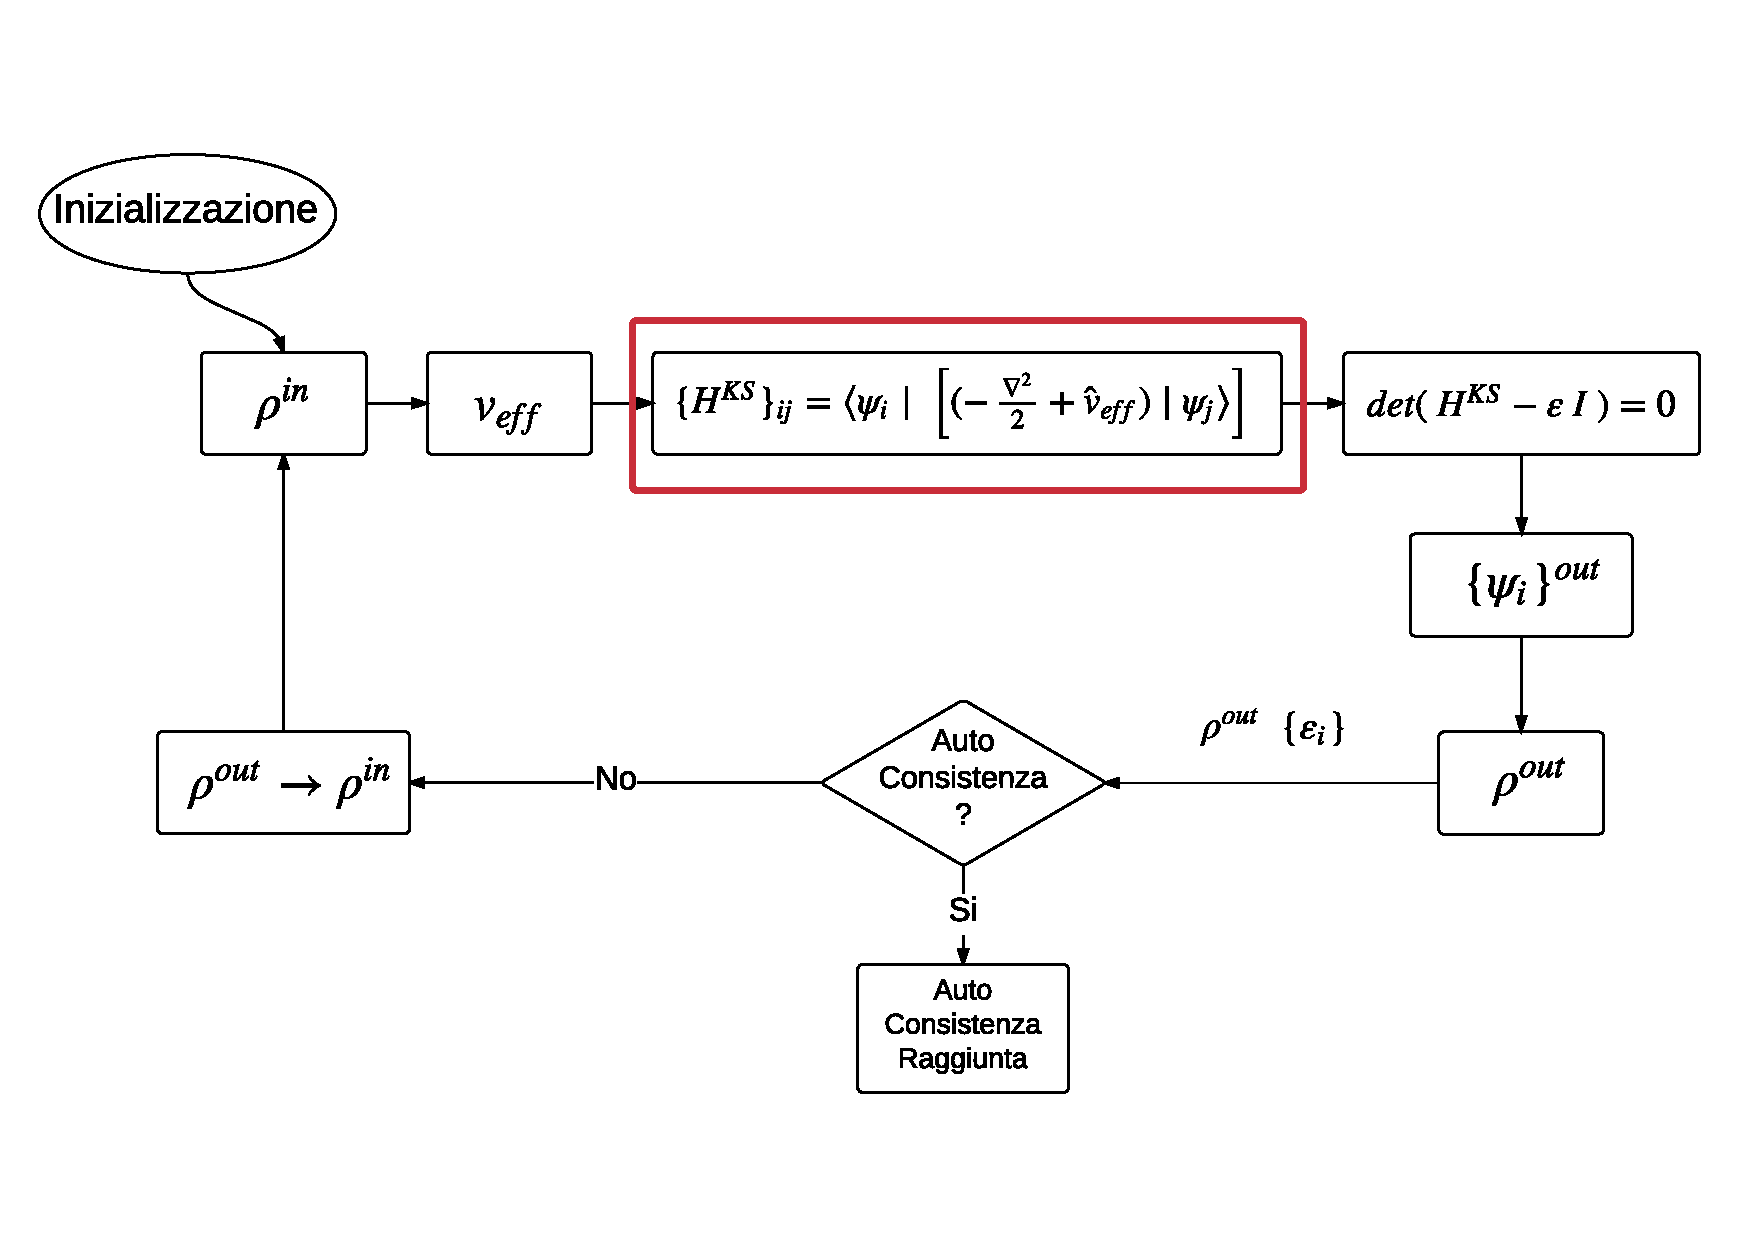
\includegraphics[height=\scfPicHeight\textheight, width=\scfPicWidth\textwidth]{beam_SCF_h_psi.pdf}	
				}
				\only<\cdiaghgPos>{
					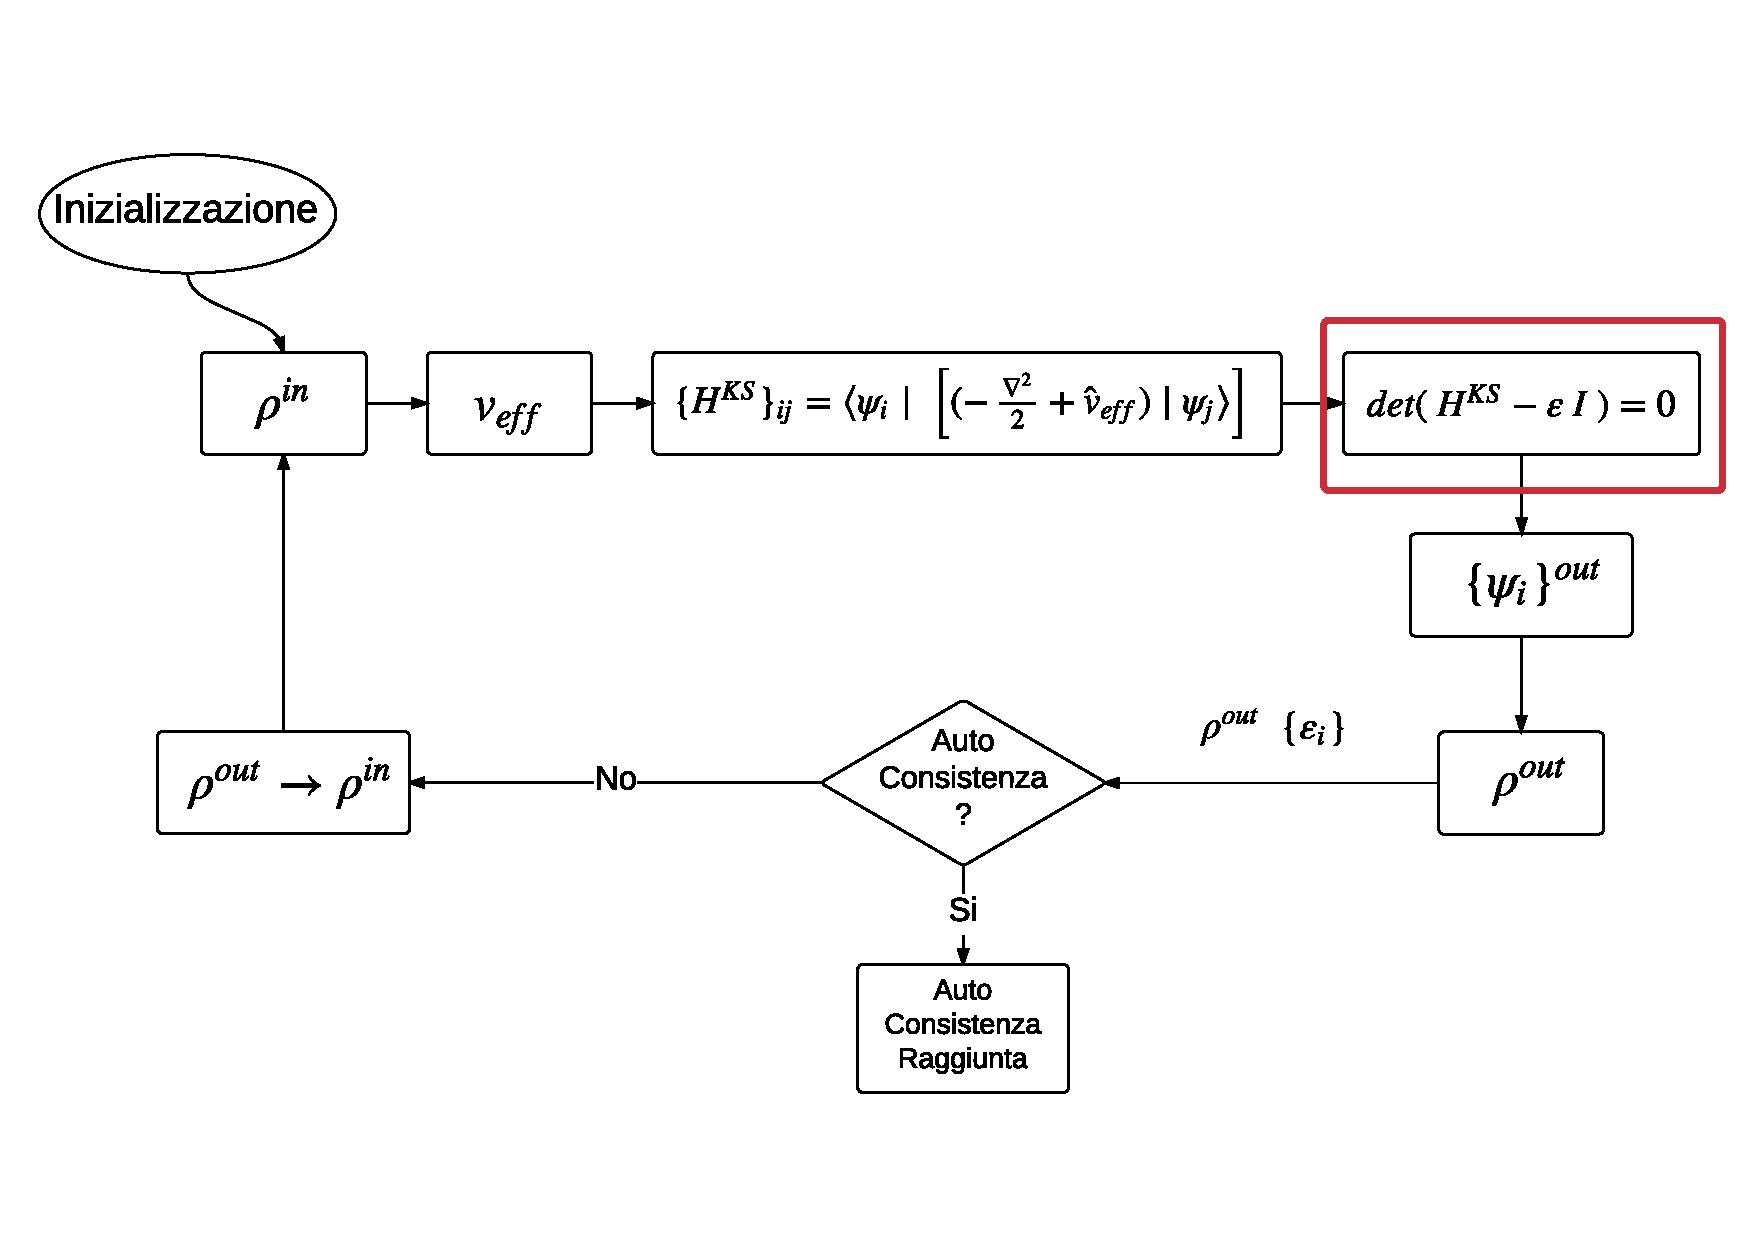
\includegraphics[height=\scfPicHeight\textheight, width=\scfPicWidth\textwidth]{beam_SCF_cdiaghg.pdf}	
				}
				\only<\sumbandPos>{
					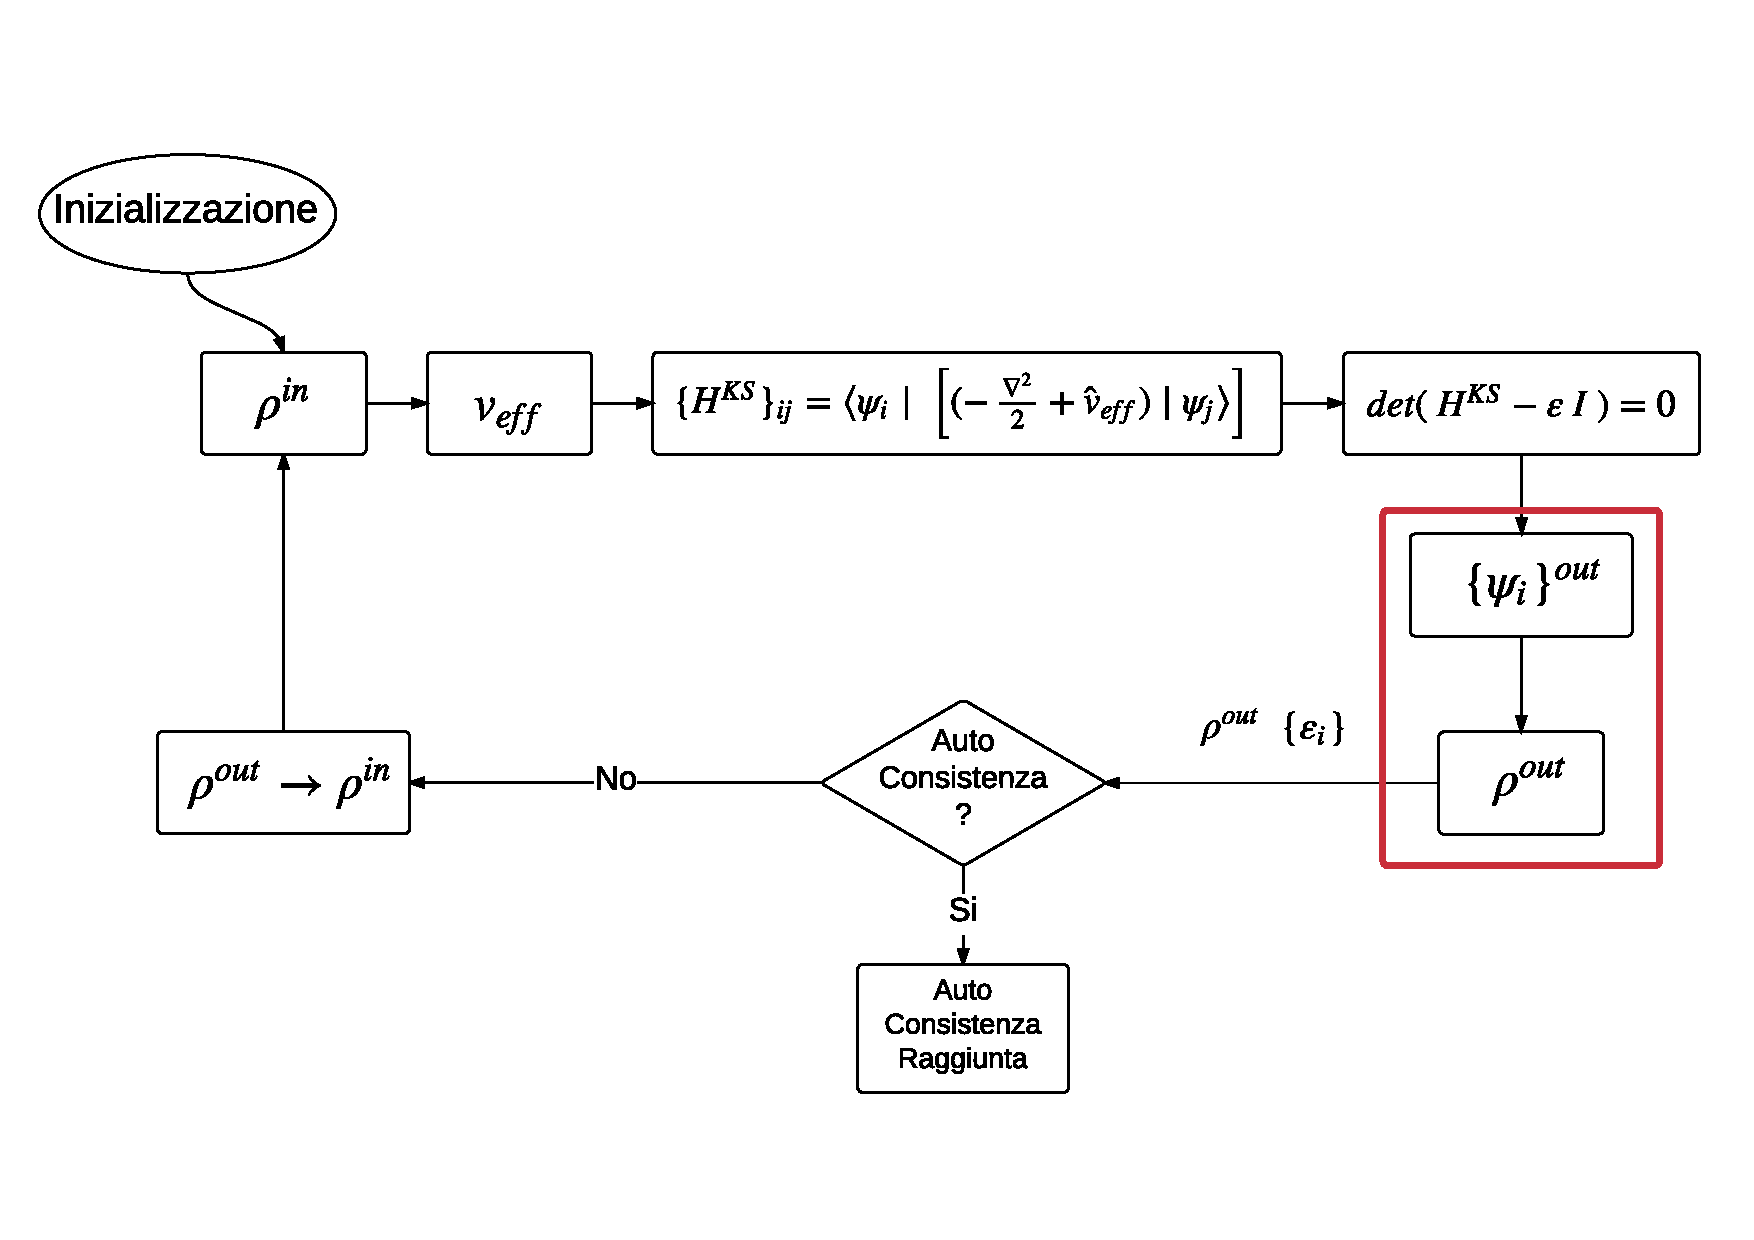
\includegraphics[height=\scfPicHeight\textheight, width=\scfPicWidth\textwidth]{beam_SCF_sum_bands.pdf}	
				}

				\end{flushleft}    	
			\column{0.5\textwidth}

				\only<1->{\vspace{-2cm}}
				
				\only<1,2>{

					\begin{block}{Pacchetto PWscf} 
						\begin{itemize}
							\item Self Consistent DFT
							\item Onde Piane come \textit{basis-set}
						\end{itemize}
					\end{block}
				}
				
				\only<\inputPos>{
					\begin{block}{Inizializzazione} 
						\begin{itemize}
							\item calcolo $\dens$ iniziale
							\item calcolo primi autovettori
							\item calcolo energia inizale
					\end{itemize}
					\end{block}
				}
				
				\only<\electronsPos>{
					\begin{block}{Problema elettronico} 
						\begin{itemize}
							\item Intero ciclo SCF
							\item Al termine si ottiene $\dens$ di ground state
					\end{itemize}
					\end{block}
				}
				\only<\cegtergPos>{
					\begin{block}{Bande elettroniche} 
						\begin{itemize}
							\item Risoluzione equazioni di Kohn-Sham\\in forma matriciale
					\end{itemize}
					\end{block}
				}
				\only<\hpsiPos>{
					\begin{block}{Valutazione Hamiltoniana} 
						\begin{itemize}
							\item Applicazione laplaciano in spazio reciproco
							\item Applicazione del potenziale in spazio reale
						\end{itemize}
					\end{block}
				}
				\only<\cdiaghgPos>{
					\begin{block}{Diagonalizzazione Hamiltoniana} 
						\begin{itemize}
							\item Algoritmo iterativo di Davidson
						\end{itemize}
					\end{block}
				}
				\only<\sumbandPos>{
					\begin{block}{Calcolo densit\`a elettronica} 
						\begin{itemize}
							\item calcolo occupazione orbitali
							\item $\displaystyle \dens = \sum_{i} f_{\psi_{i}} ~ \psi_{i}^{*KS}(\erre) ~ \psi_{i}^{KS}(\erre)$
						\end{itemize}
					\end{block}
				}
				\only<\fftPos,\fftscatterPos>{
					\begin{block}{Moduli generici} 
						\begin{itemize}
							\visible<\fftPos,\fftscatterPos>{\item Calcolo FFT}
							\visible<\fftscatterPos>{\item Distribuzione griglia}

						\end{itemize}
					\end{block}
				}
				
    	\end{columns}

    \end{minipage}

    \nointerlineskip
    \begin{minipage}[b][0.5\textheight][t]{\textwidth}
        	\begin{columns}
			\column{0.5\textwidth}
				
			\column{0.5\textwidth}
				\vspace{-1cm}
				\begin{center}
			   	\only<1>{
					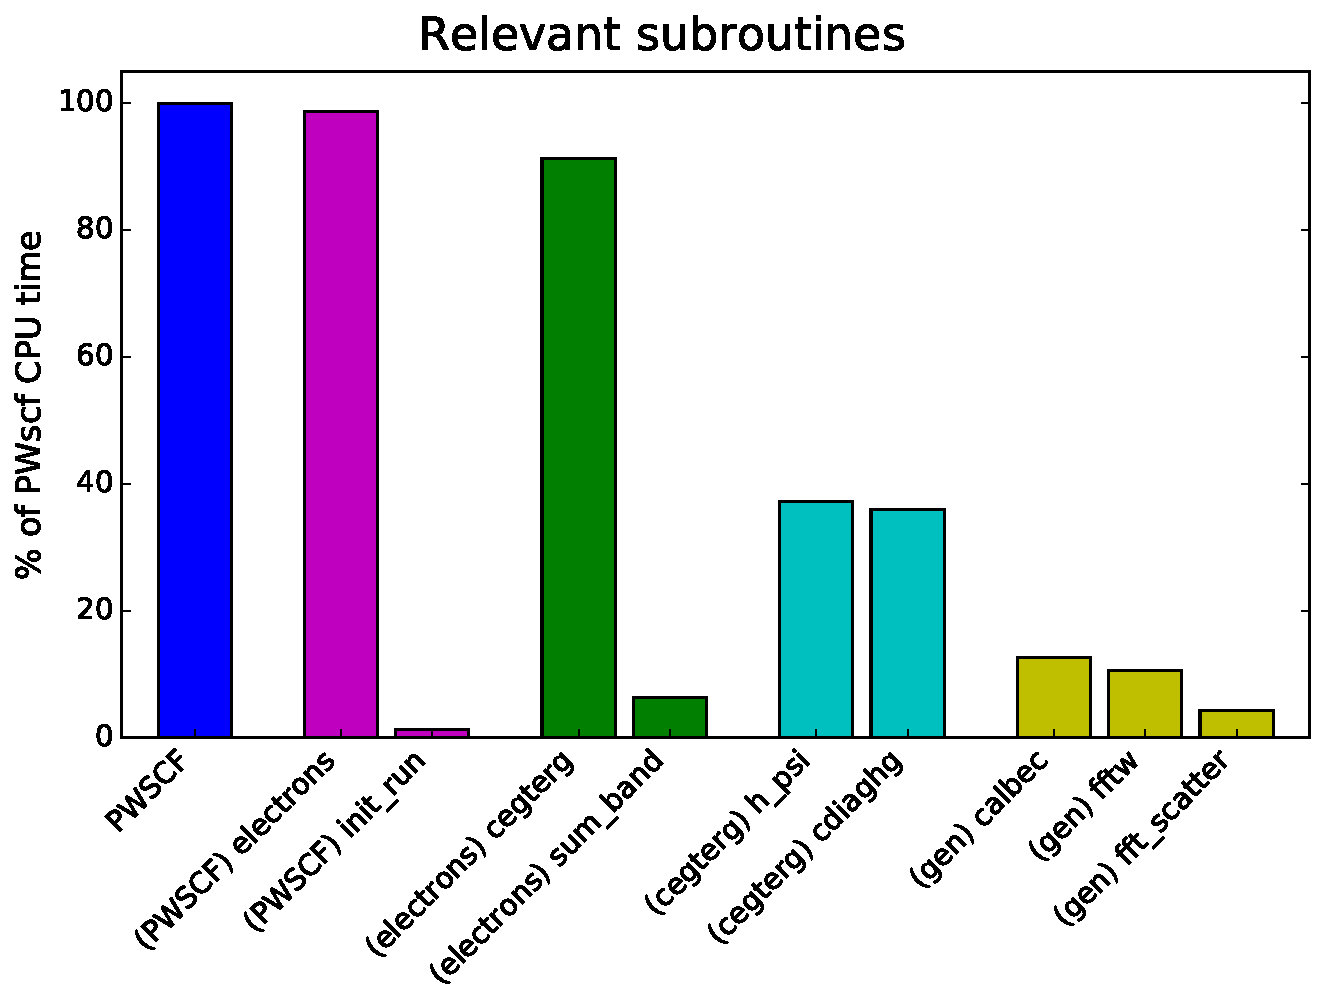
\includegraphics[height=0.5\textheight, width=1\textwidth]{beam_relevant_subroutines.pdf}	
				}
				\only<2>{
					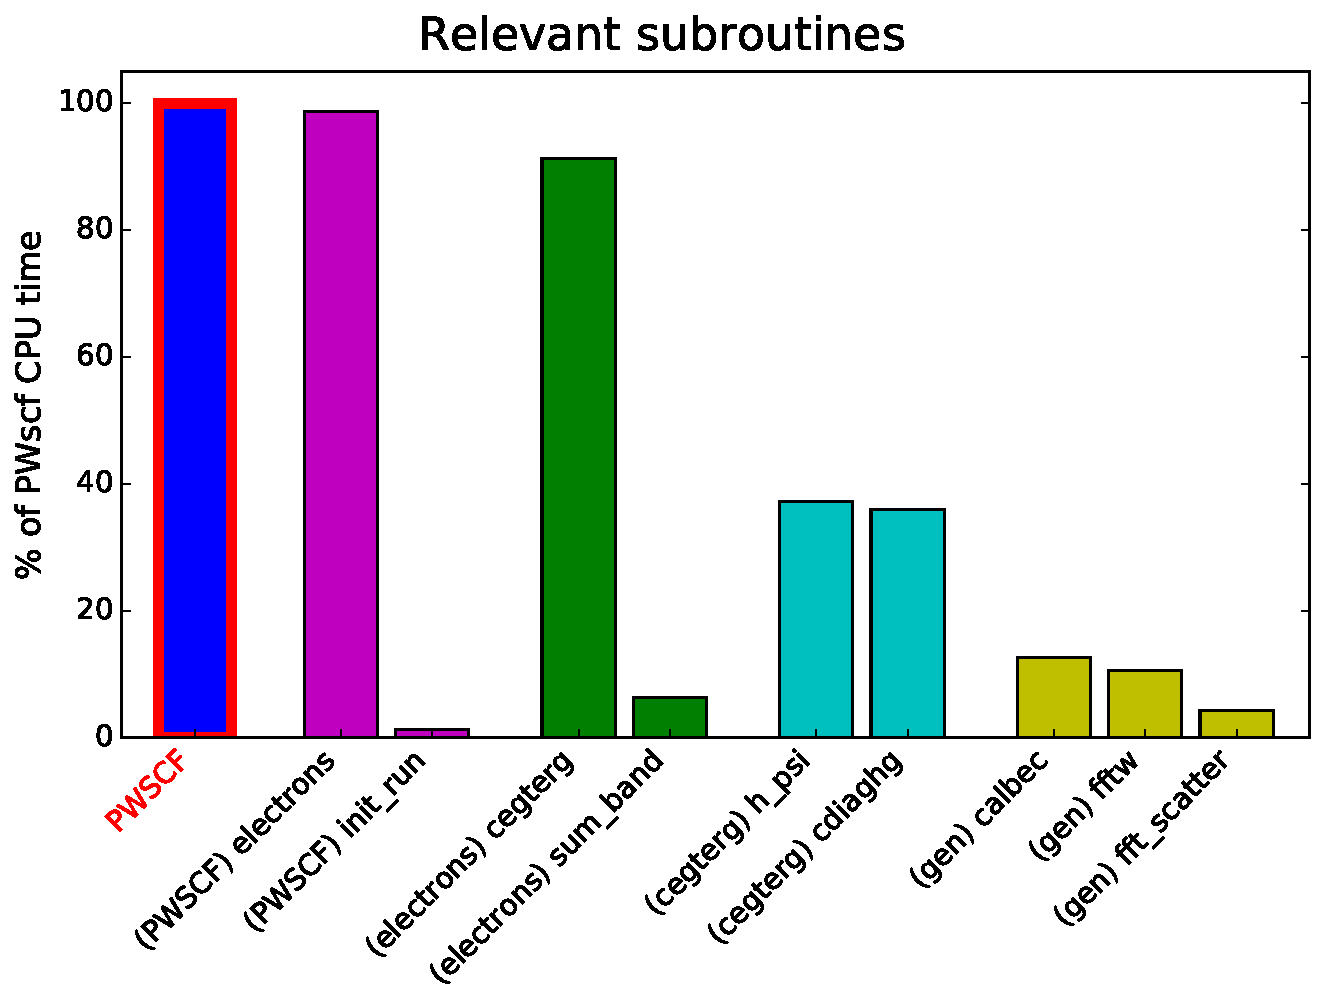
\includegraphics[height=0.5\textheight, width=1\textwidth]{beam_relevant_subroutines_PWSCF.pdf}	
				}
				\only<3>{
					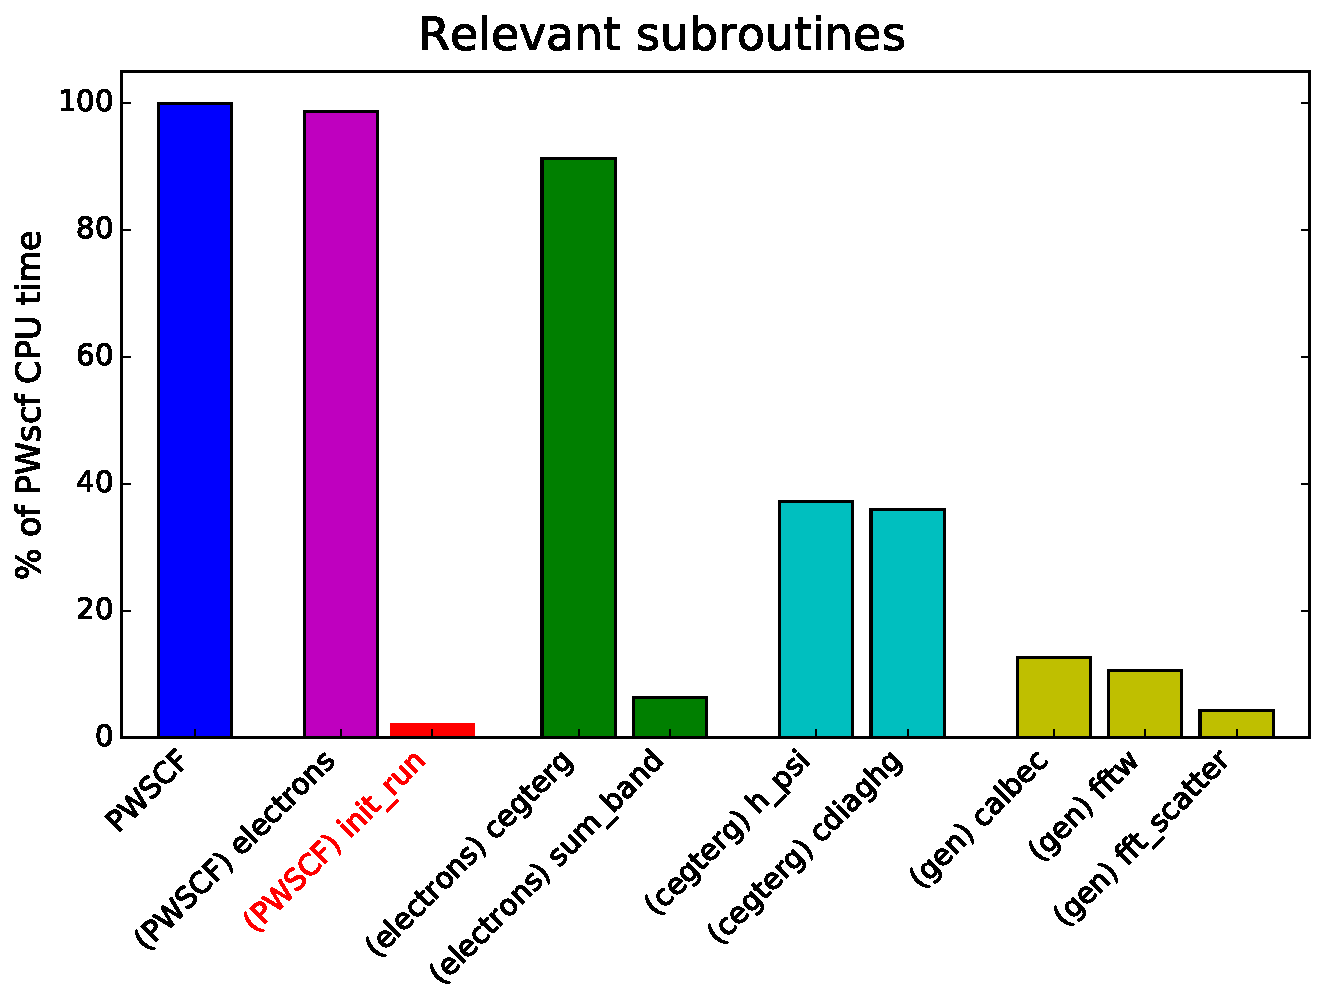
\includegraphics[height=0.5\textheight, width=1\textwidth]{beam_relevant_subroutines_init_run.pdf}	
				}
				\only<4>{
					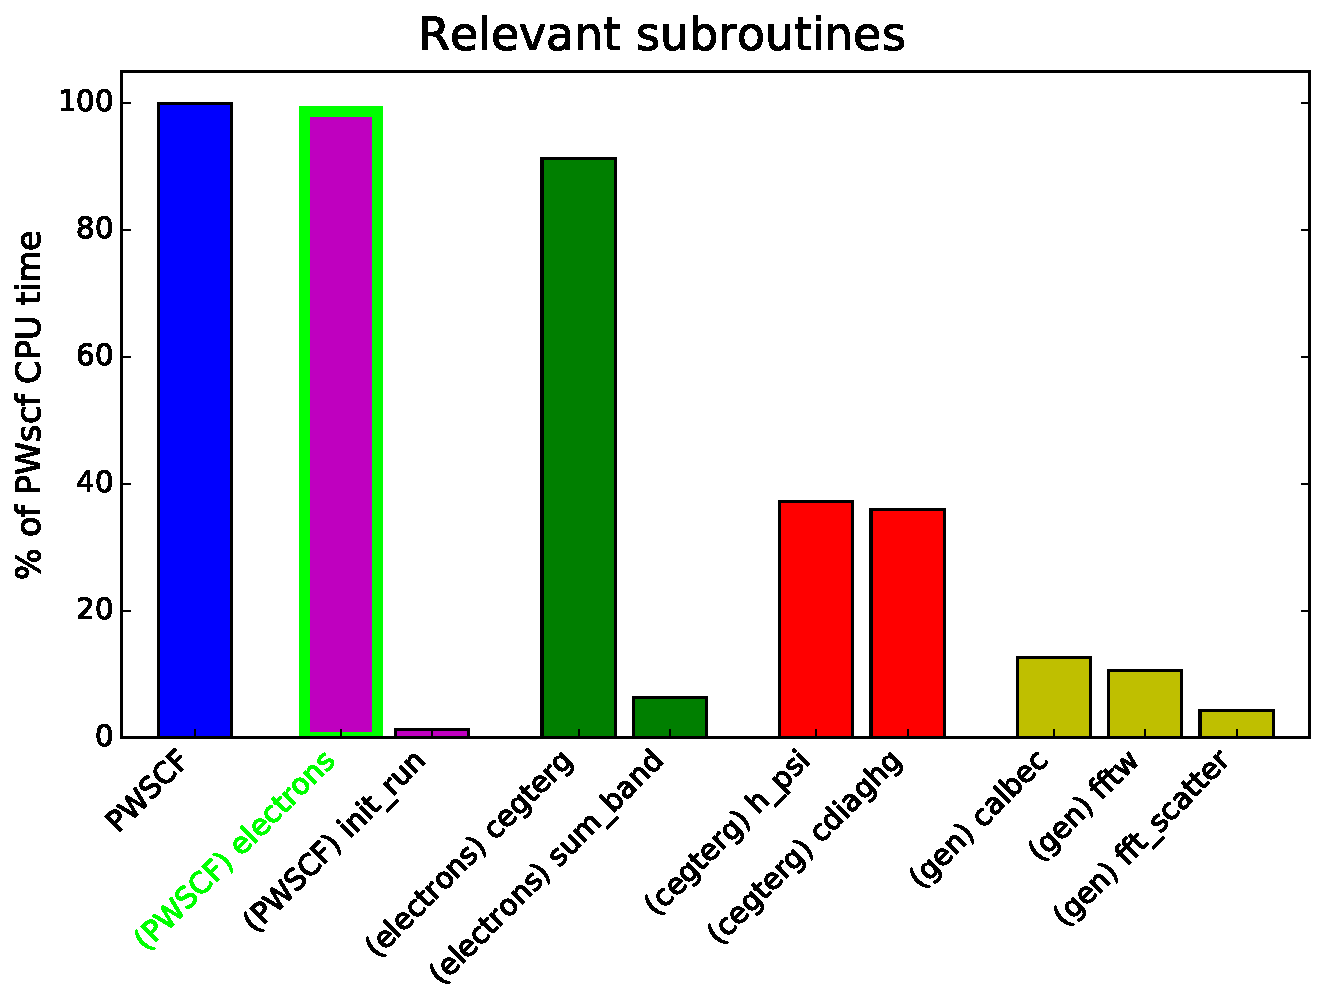
\includegraphics[height=0.5\textheight, width=1\textwidth]{beam_relevant_subroutines_electrons.pdf}	
				}
				\only<5>{
					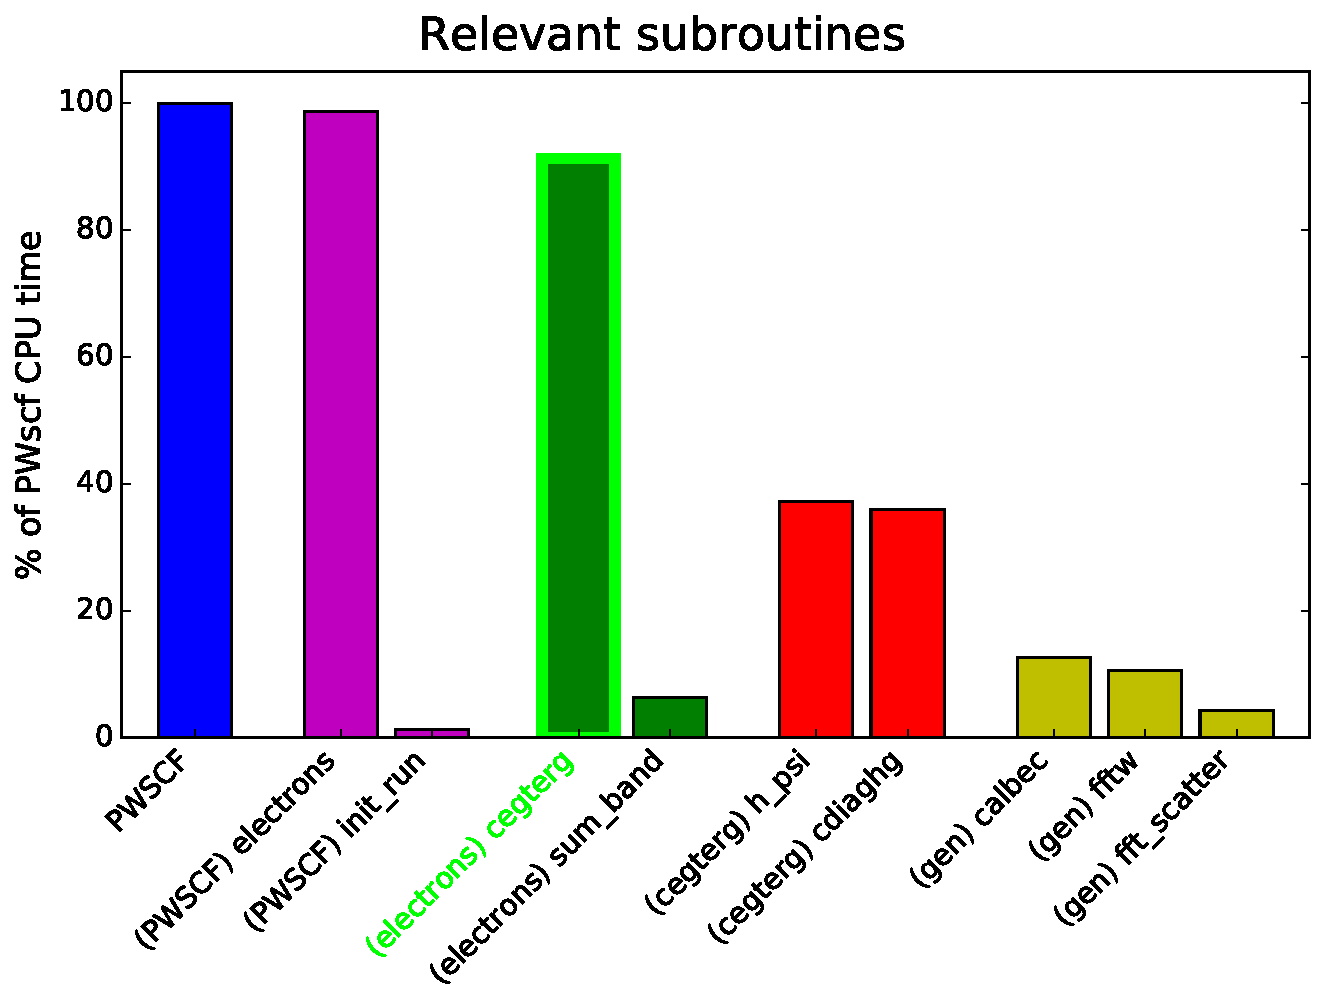
\includegraphics[height=0.5\textheight, width=1\textwidth]{beam_relevant_subroutines_cegterg.pdf}	
				}
				\only<6>{
					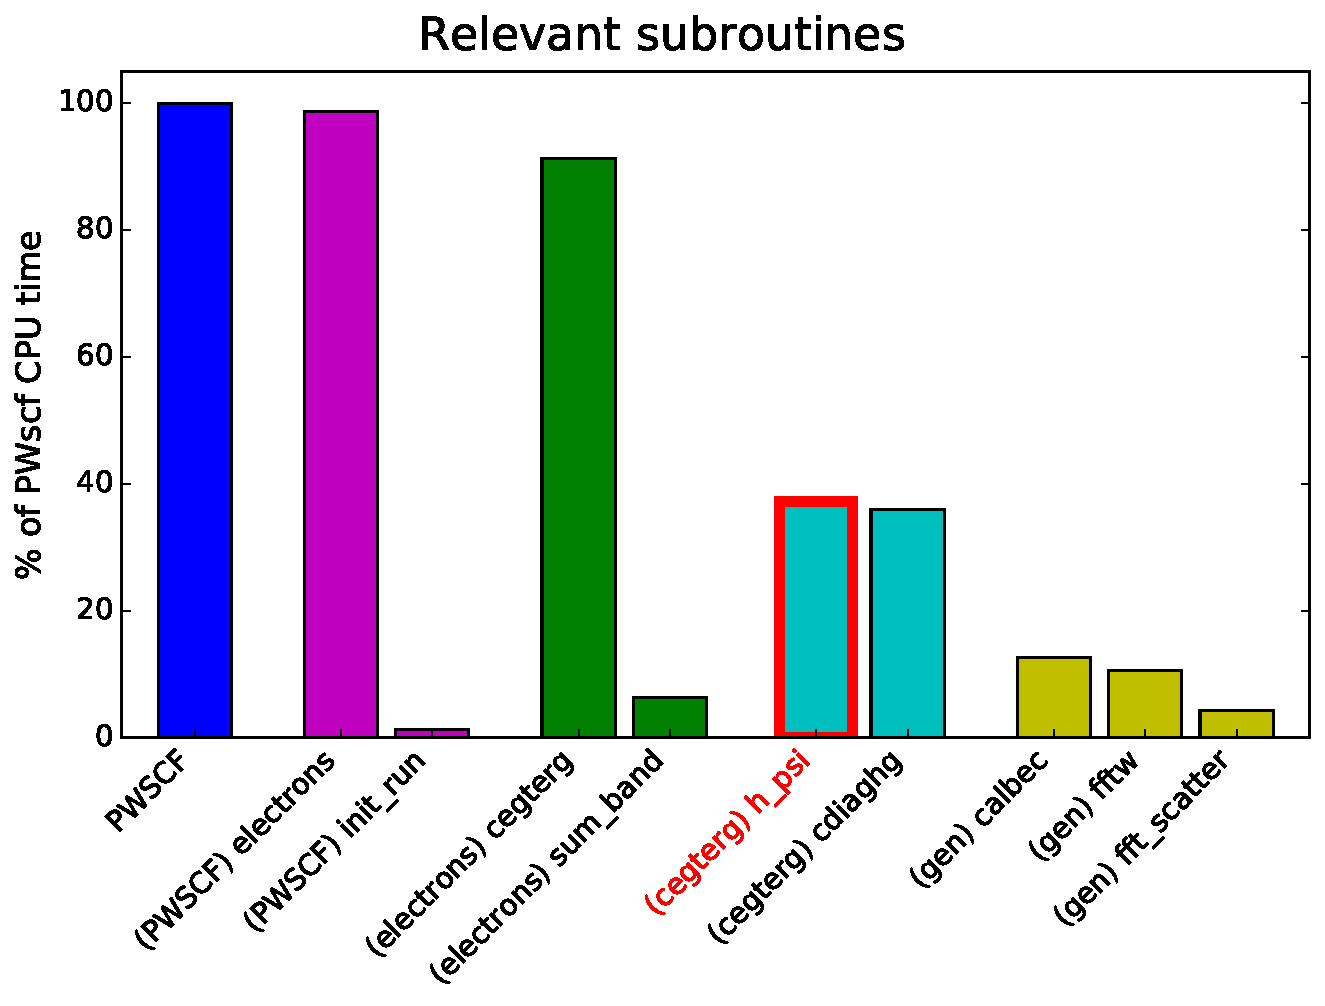
\includegraphics[height=0.5\textheight, width=1\textwidth]{beam_relevant_subroutines_h_psi.pdf}	
				}
				\only<7>{
					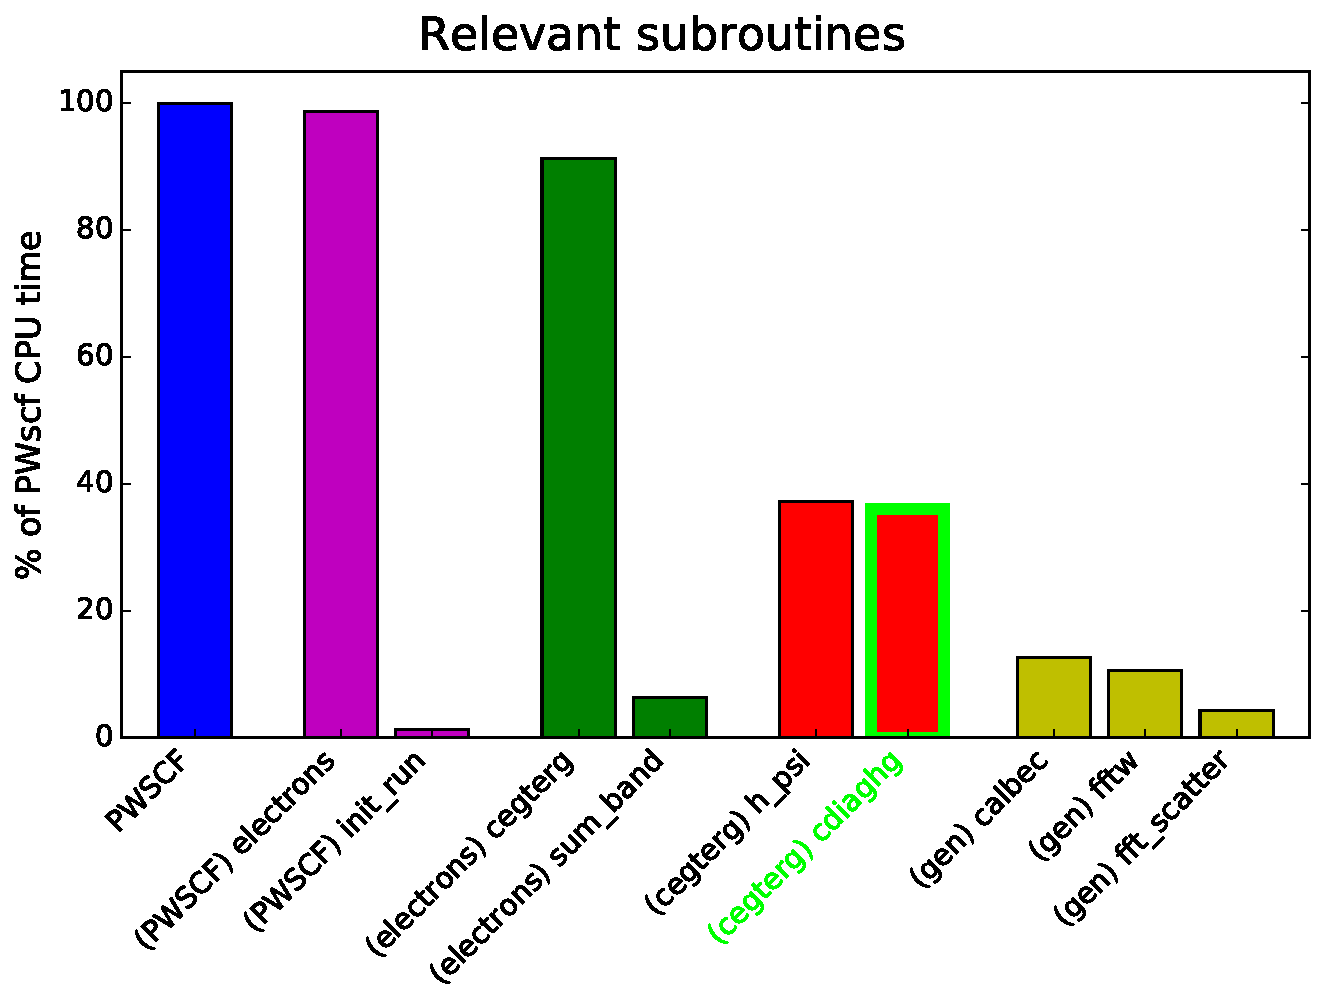
\includegraphics[height=0.5\textheight, width=1\textwidth]{beam_relevant_subroutines_cdiaghg.pdf}	
				}				
				\only<8>{
					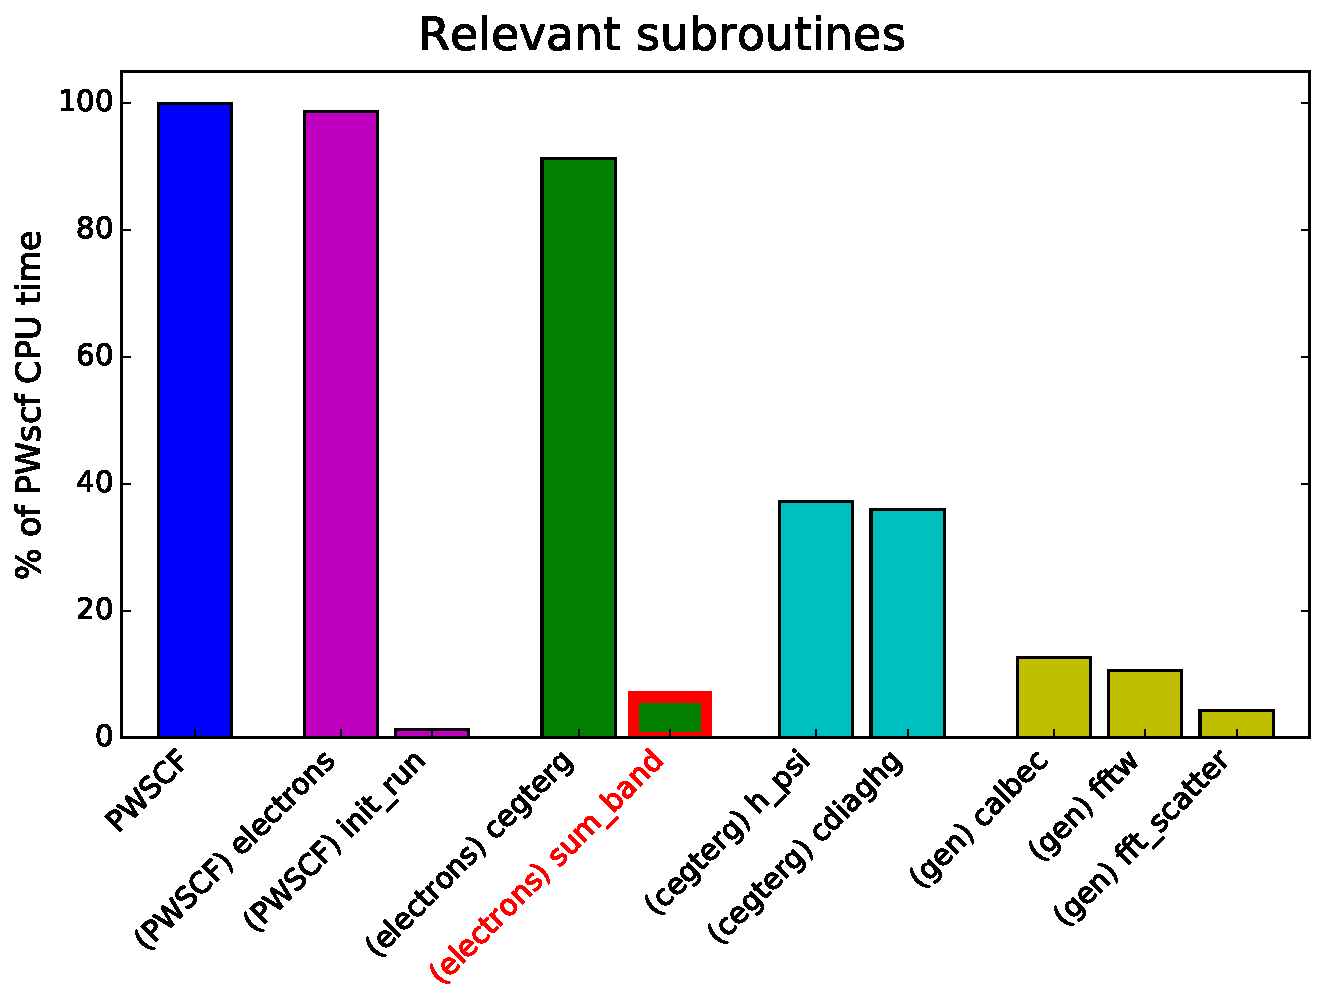
\includegraphics[height=0.5\textheight, width=1\textwidth]{beam_relevant_subroutines_sum_band.pdf}	
				}
				\only<9>{
					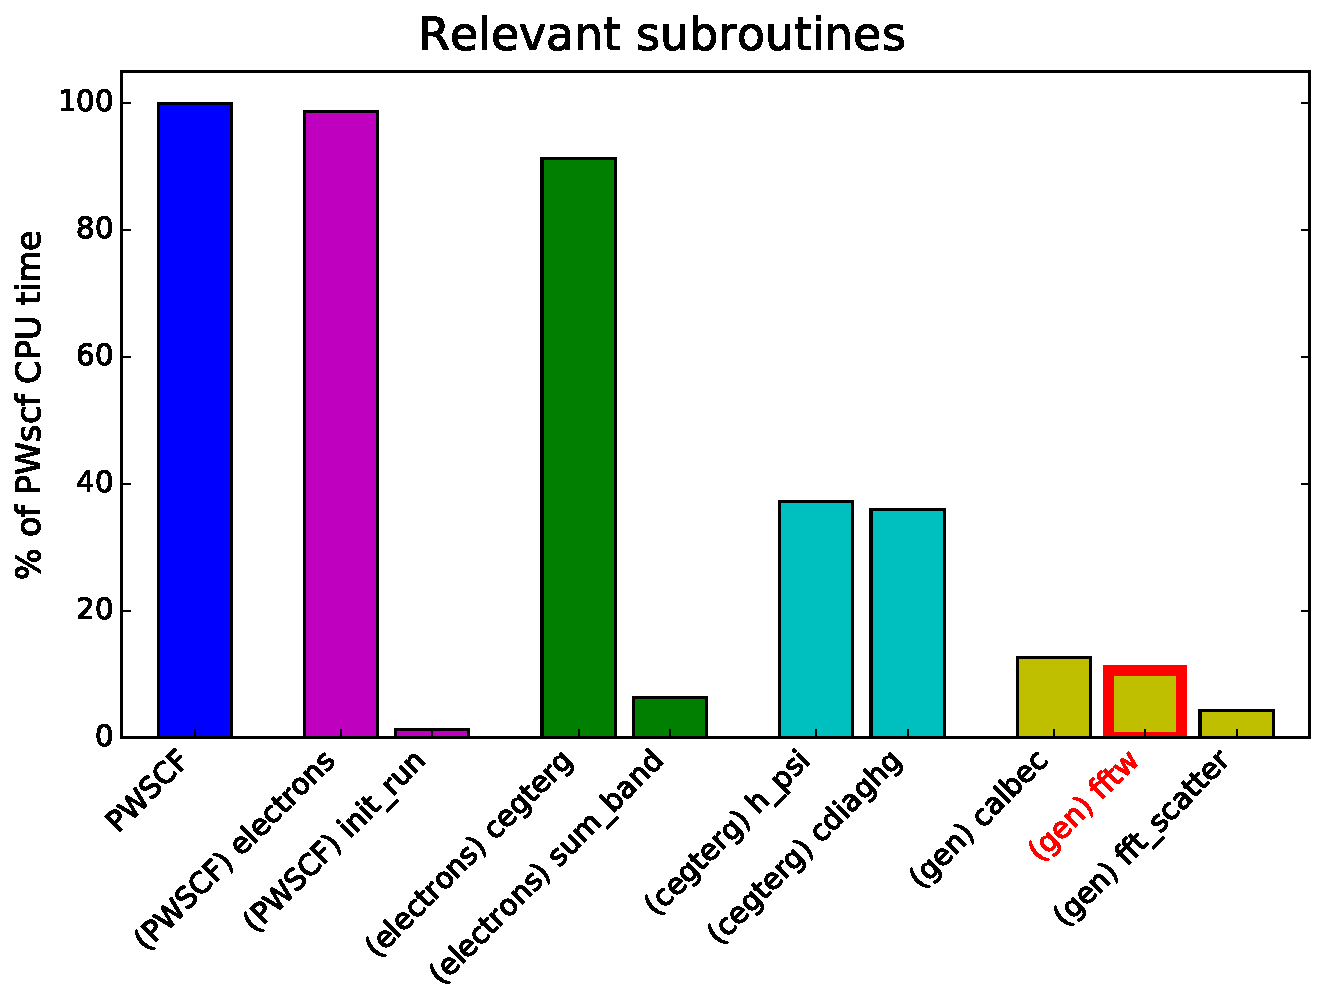
\includegraphics[height=0.5\textheight, width=1\textwidth]{beam_relevant_subroutines_fftw.pdf}	
				}
				\only<10>{
					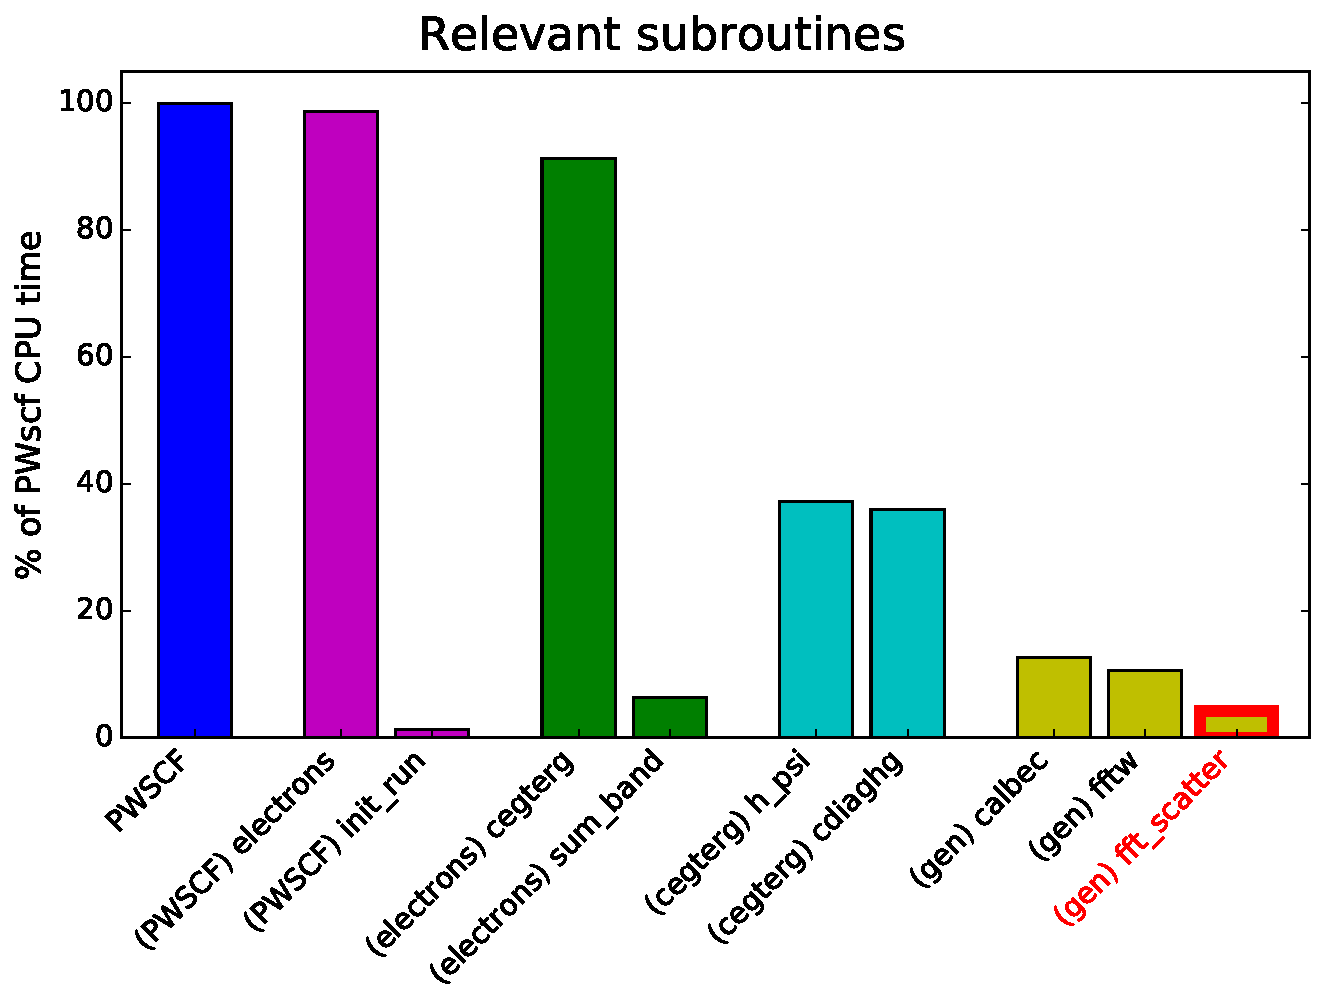
\includegraphics[height=0.5\textheight, width=1\textwidth]{beam_relevant_subroutines_fft_scatter.pdf}	
				}
				\end{center}    	
    	\end{columns}

    \end{minipage}
}

\end{frame}


% ********** slide 6 *****************}
\section{Architetture computazionali}
\subsection{Architetture computazionali}
\begin{frame}{Cluster Infiniband}

\begin{columns}
	\column{0.5\textwidth}
	\begin{block}{CINECA Galileo cluster}
		\begin{itemize}
			\item Architettura multicomputer
			\item Ogni nodo indipendente
			\item 16 core per nodo divisi su due socket
			\item Interconnect Infiniband
		\end{itemize}
	\end{block}

	\column{0.5\textwidth}
			\begin{center}
				schema CLUSTER
			\end{center}
\end{columns}

\end{frame}

% ********** slide 7 *****************}
\begin{frame}{Macchina a memoria condivisa}
\begin{columns}
	\column{0.5\textwidth}
	\begin{block}{Sgi Altix UV2000 CC-NUMA}
		\begin{itemize}
			\item Architettura multiprocessore
			\item Unica macchina a memoria condivisa
			\item 8 core per nodo numa
			\item 64 core totali
		\end{itemize}
	\end{block}
	
	\column{0.5\textwidth}
	\begin{center}
		schema NUMA
	\end{center}
	
\end{columns}

\end{frame}


% ********** slide 9 *****************}

\section{Risultati}
\subsection{Risultati}

\begin{frame}{Risultati}
\begin{columns}
	\visible<1->{
	\column{0.5\textwidth}
		\begin{block}{Indipendenti dall'architettura}
			\begin{itemize}
				\item Su singolo nodo
				%\item Bassa parallelizzazione
				\item Basso numero di core
				\item No interconnect
			\end{itemize}
		\end{block}
	}
	\visible<1->{
	\column{0.5\textwidth}
		\begin{block}{Dipendenti dall'architettura}
			\begin{itemize}
				\item Nodi multipli
				\item Alta parallelizzazione
				%\item Alto numero di core
				\item Interconnect o memoria condivisa
			\end{itemize}
		\end{block}
	}
\end{columns}
\begin{center}
	\visible<2->{
	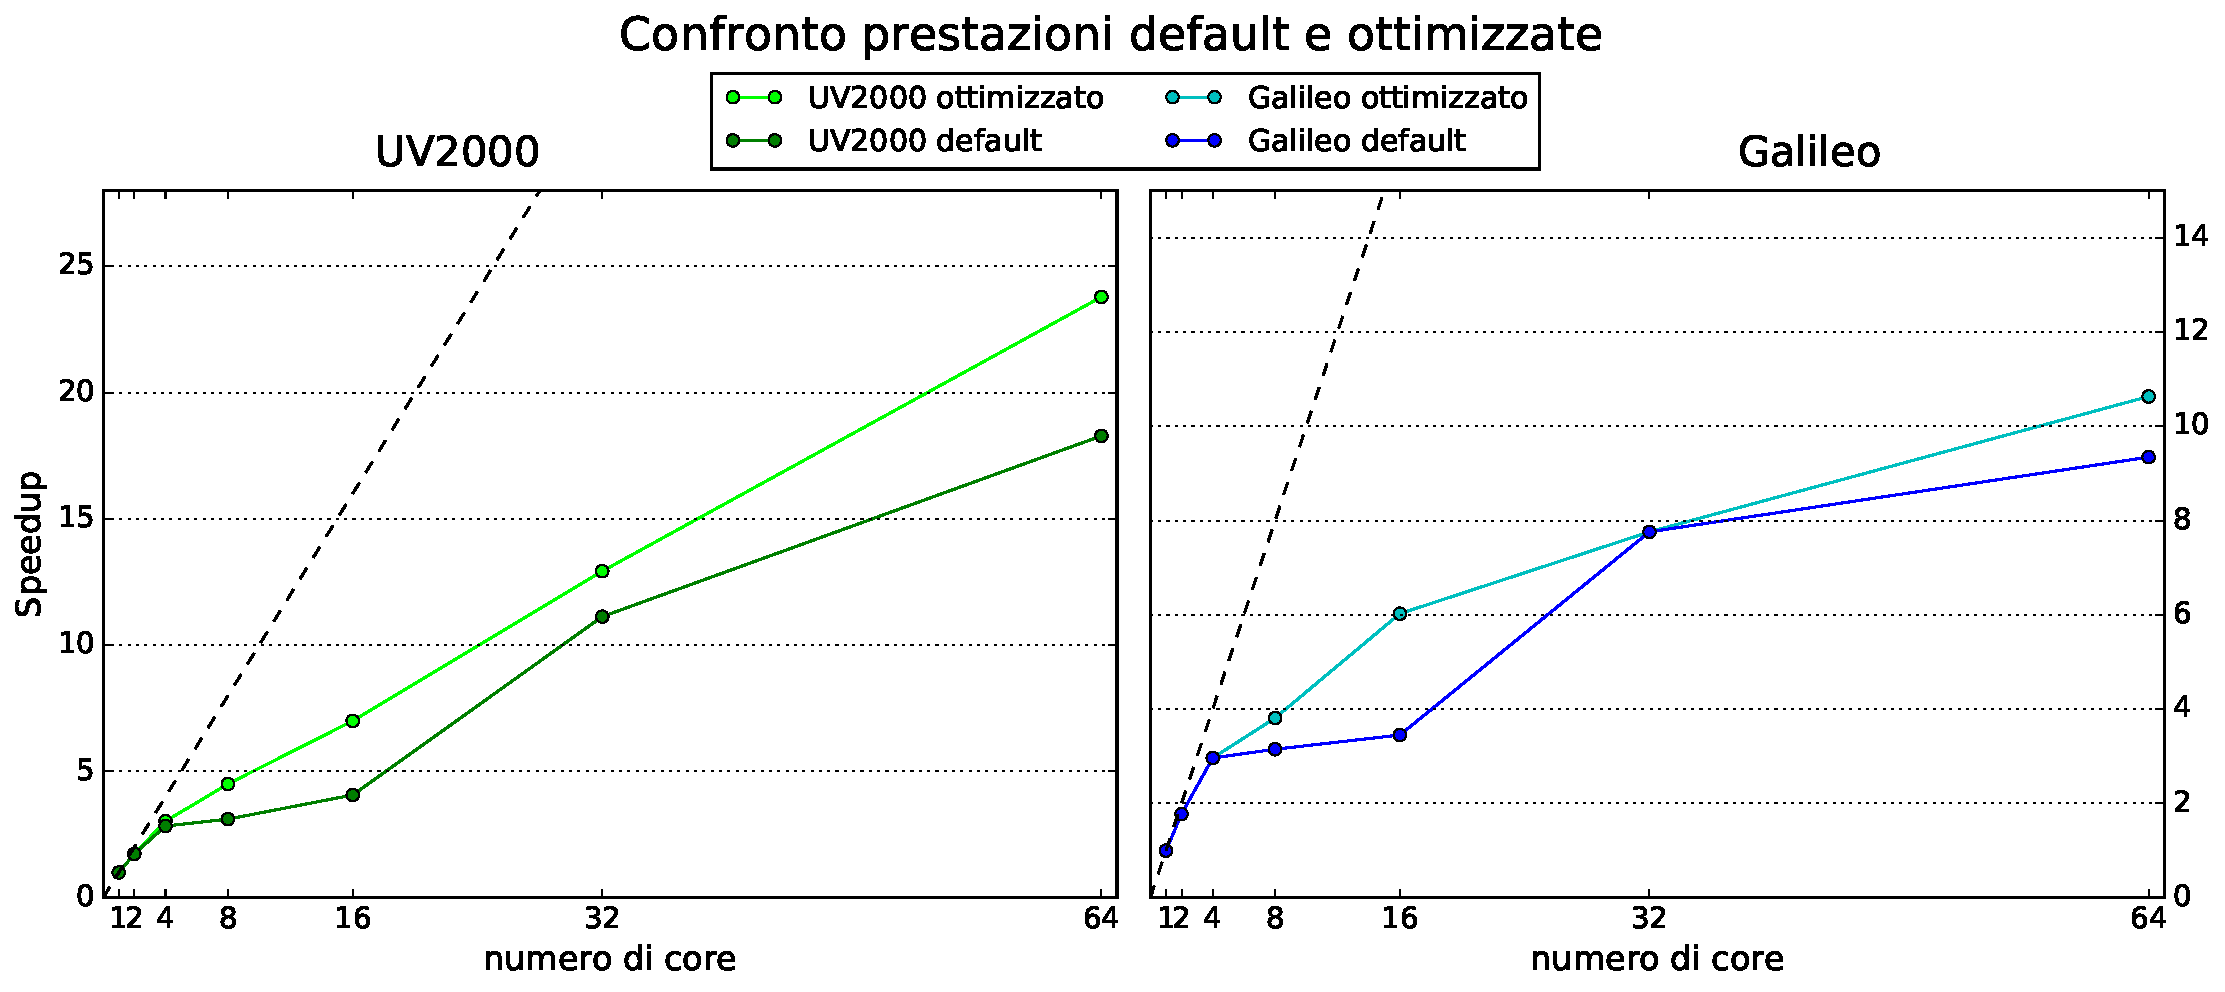
\includegraphics[height=0.6\textheight]{beam_results_arch_comparison.pdf}	
	}
\end{center}
\end{frame}



% ********** slide 10 *****************}

\begin{frame}{Indipendenti dall'architettura}

\begin{columns}[c]

\column{0.5\textwidth}
\parbox[c]{0.5\linewidth}
{
\begin{center}
	\only<1>{
	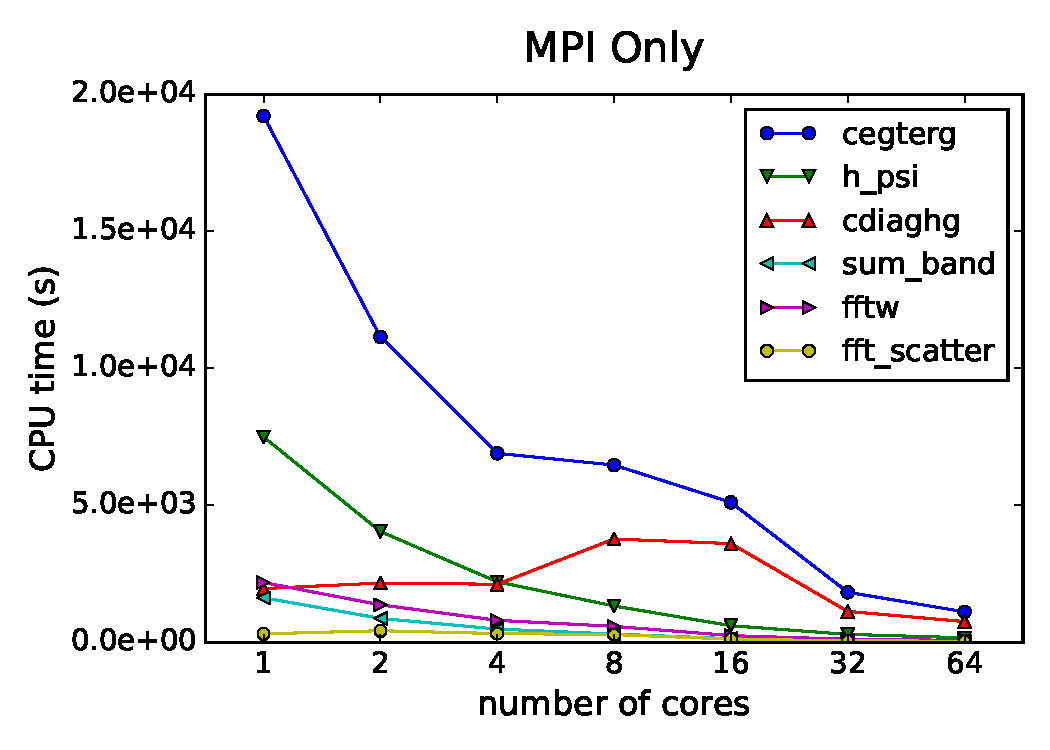
\includegraphics[width=1\textwidth, height=0.5 \textheight]{beam_threads_MPIonly.pdf}	
	}
	\only<2>{
	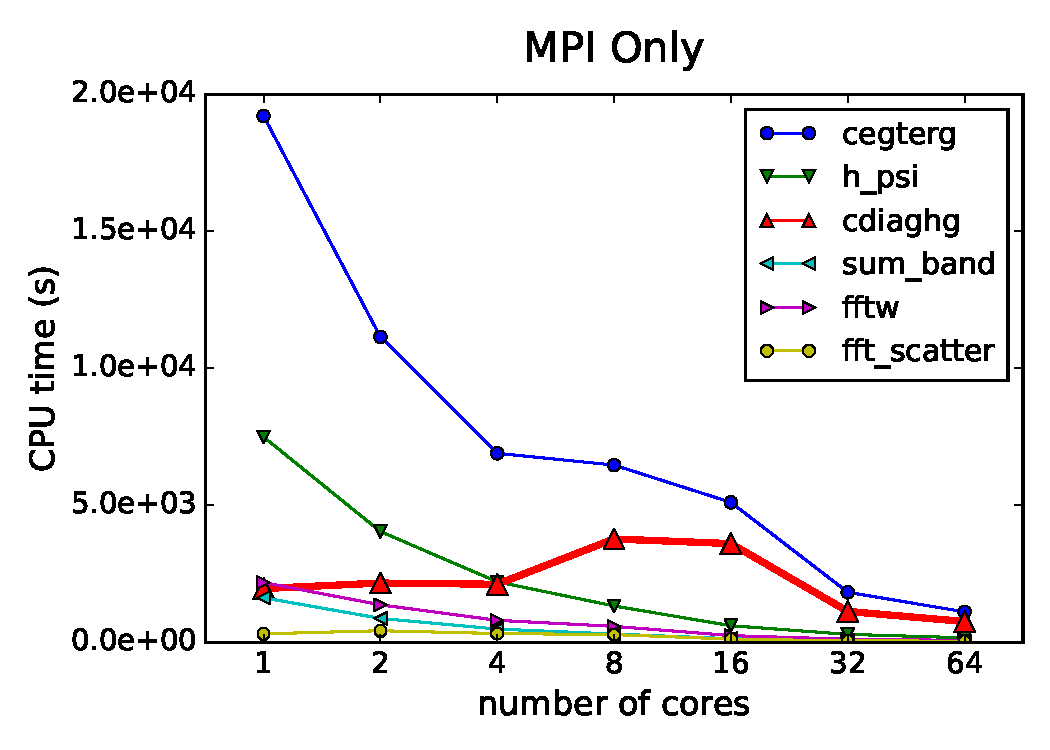
\includegraphics[width=1\textwidth, height=0.5 \textheight]{beam_threads_MPIonly_cdiaghg.pdf}	
	}
	%\only<3>{
	%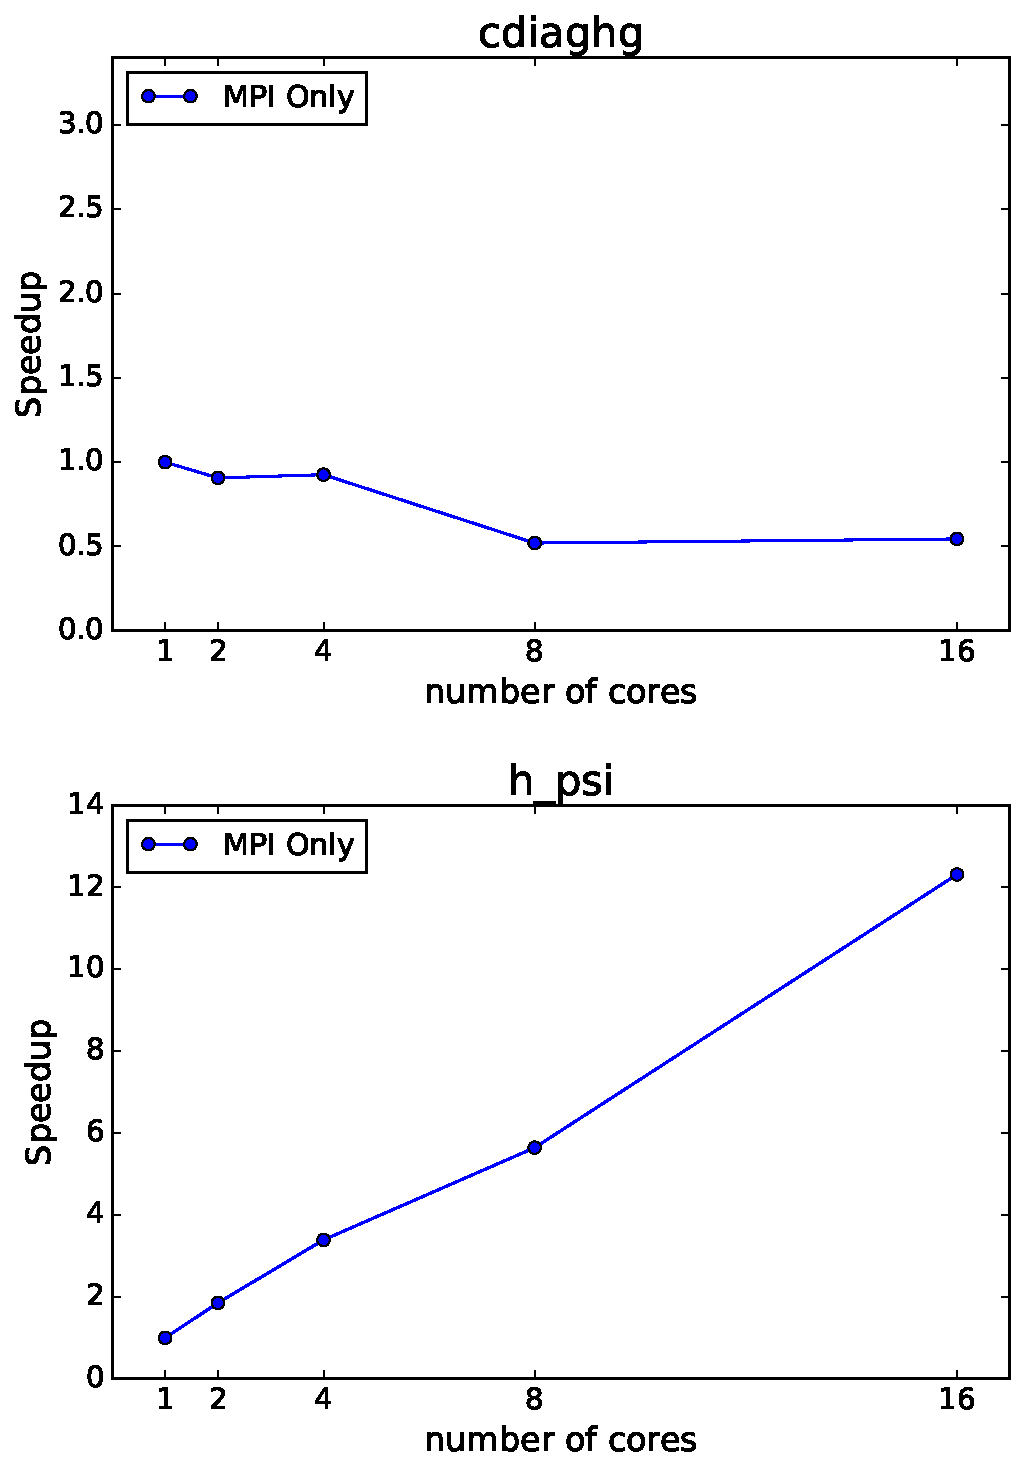
\includegraphics[width=0.9\textwidth, height=0.85 \textheight]{beam_threads_subroutines_MPI.pdf}	
	%}
	\only<3->{
	\vspace{-1cm}
	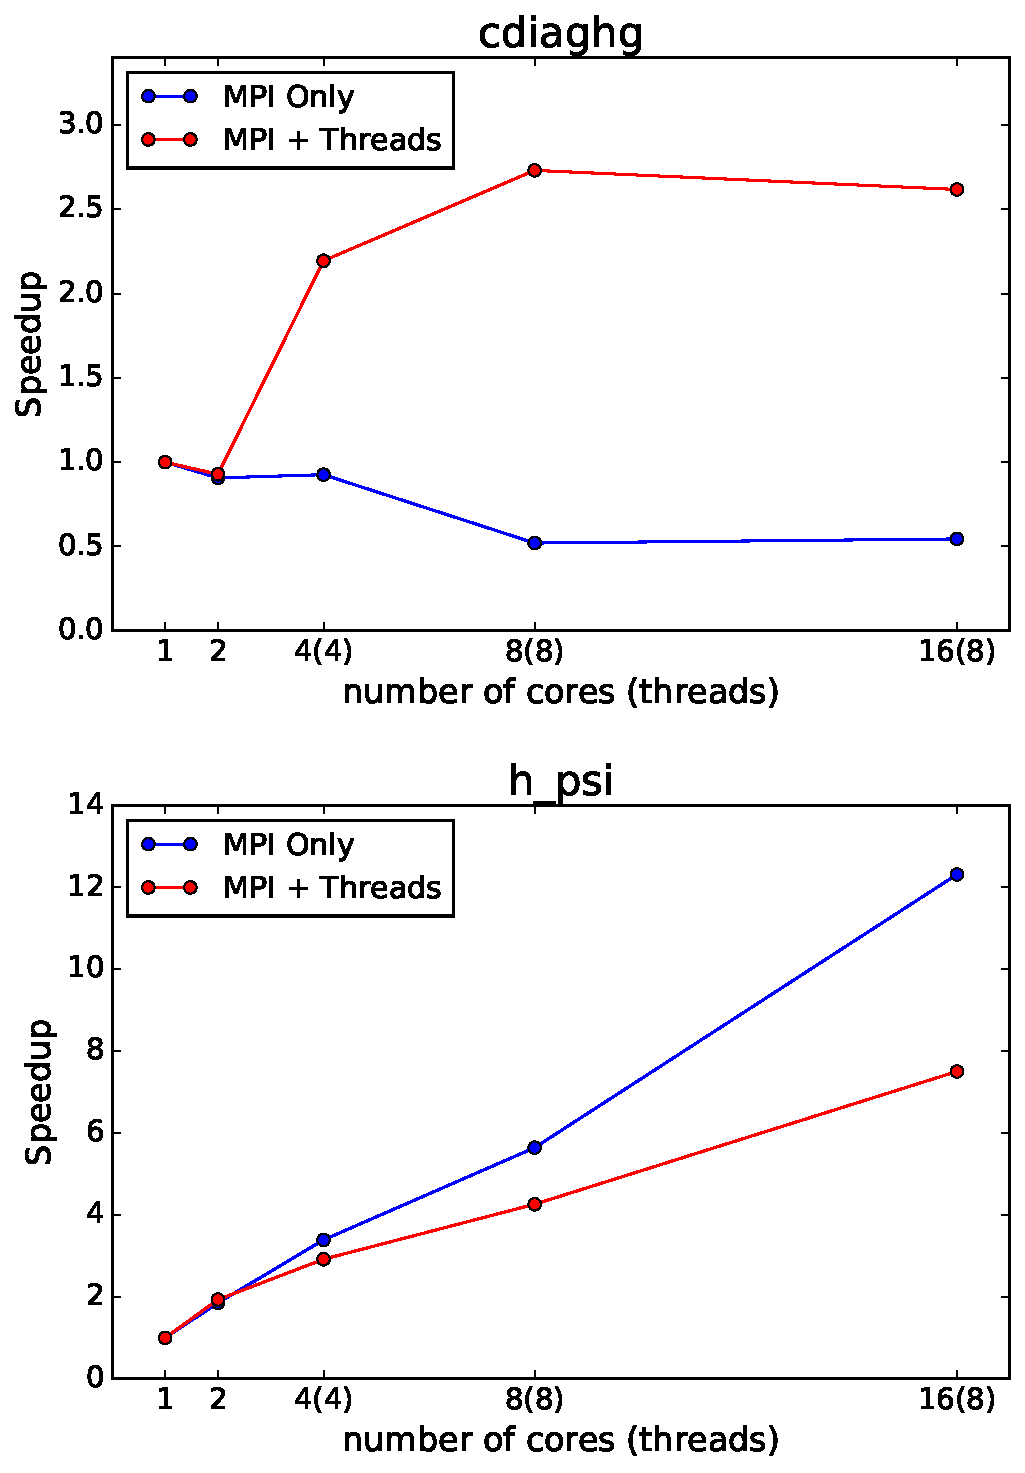
\includegraphics[width=0.9\textwidth, height=0.85 \textheight]{beam_threads_subroutines_MPI_threads.pdf}	
	}
\end{center}
}

\column{0.5\textwidth}
\begin{center}
\begin{overlayarea}{\linewidth}{\textheight}


	\begin{block}{Comportamento}
		\begin{itemize}
			\item<1-> MPI: parallelizzazione multiprocesso a memoria distribuita
			\item<2-> Diagonalizzazione ScaLapack poco performante
			\item<3-> Threads forzano diagonalizzazione con MKL
			\item<4-> Valutazione Hamiltoniana rallenta ma diagonalizzazione \`e pi\`u efficiente
			\item<5-> Risultato?
		\end{itemize}
	\end{block}

\end{overlayarea}
\end{center}

\end{columns}


\end{frame}


% ********** slide 11 *****************}
\begin{frame}{Indipendenti dall'Architettura}
	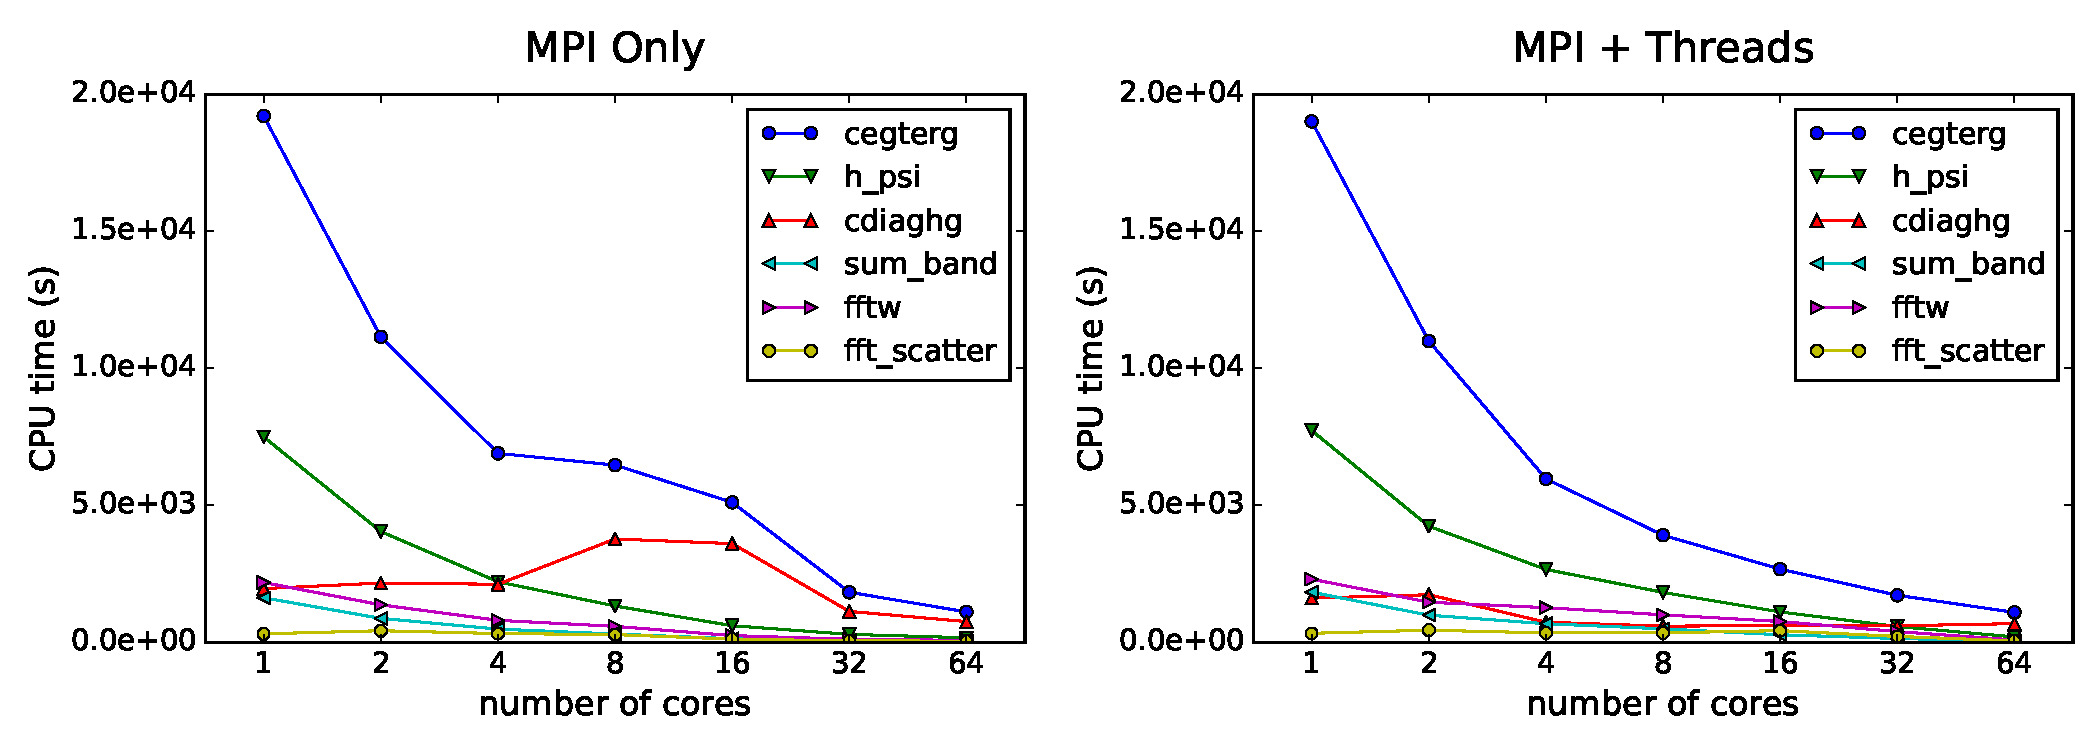
\includegraphics[width=1\textwidth]{threads_comparison.pdf}	
\end{frame}



% ********** slide 12 *****************}
\begin{frame}{Dipendenti dall'architettura}
\begin{columns}
	\column{0.5\textwidth}
			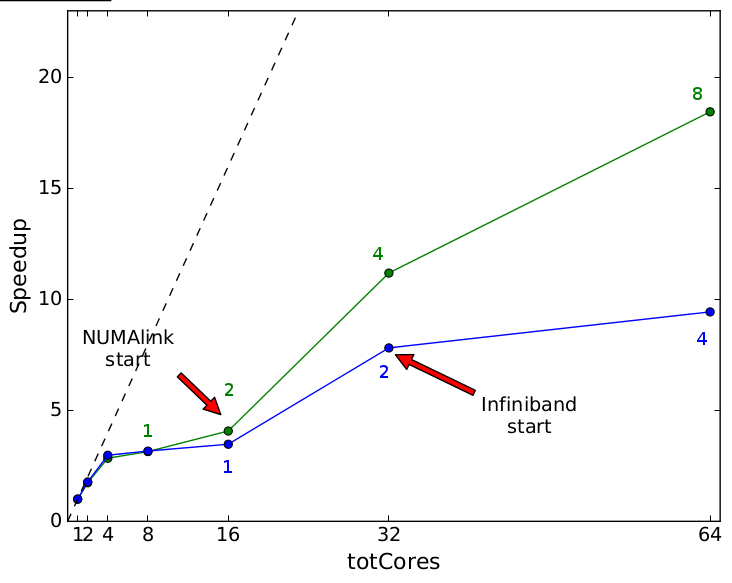
\includegraphics[width=1\textwidth]{beam_arch_global.jpg}			
	\column{0.5\textwidth}
		\begin{block}{Confronto Architetture}
			\begin{itemize}
				\item UV2000 miglior scaling
				\item Differenza cresce all'aumentare dei nodi
				\item Andamento funzioni?		
			\end{itemize}
		\end{block}
\end{columns}
\end{frame}

% ********** slide 13 *****************}
\begin{frame}{Dipendenti dall'architettura}
\begin{columns}
	\column{0.66\textwidth}
		\begin{center}			
			\vspace{-1cm}
			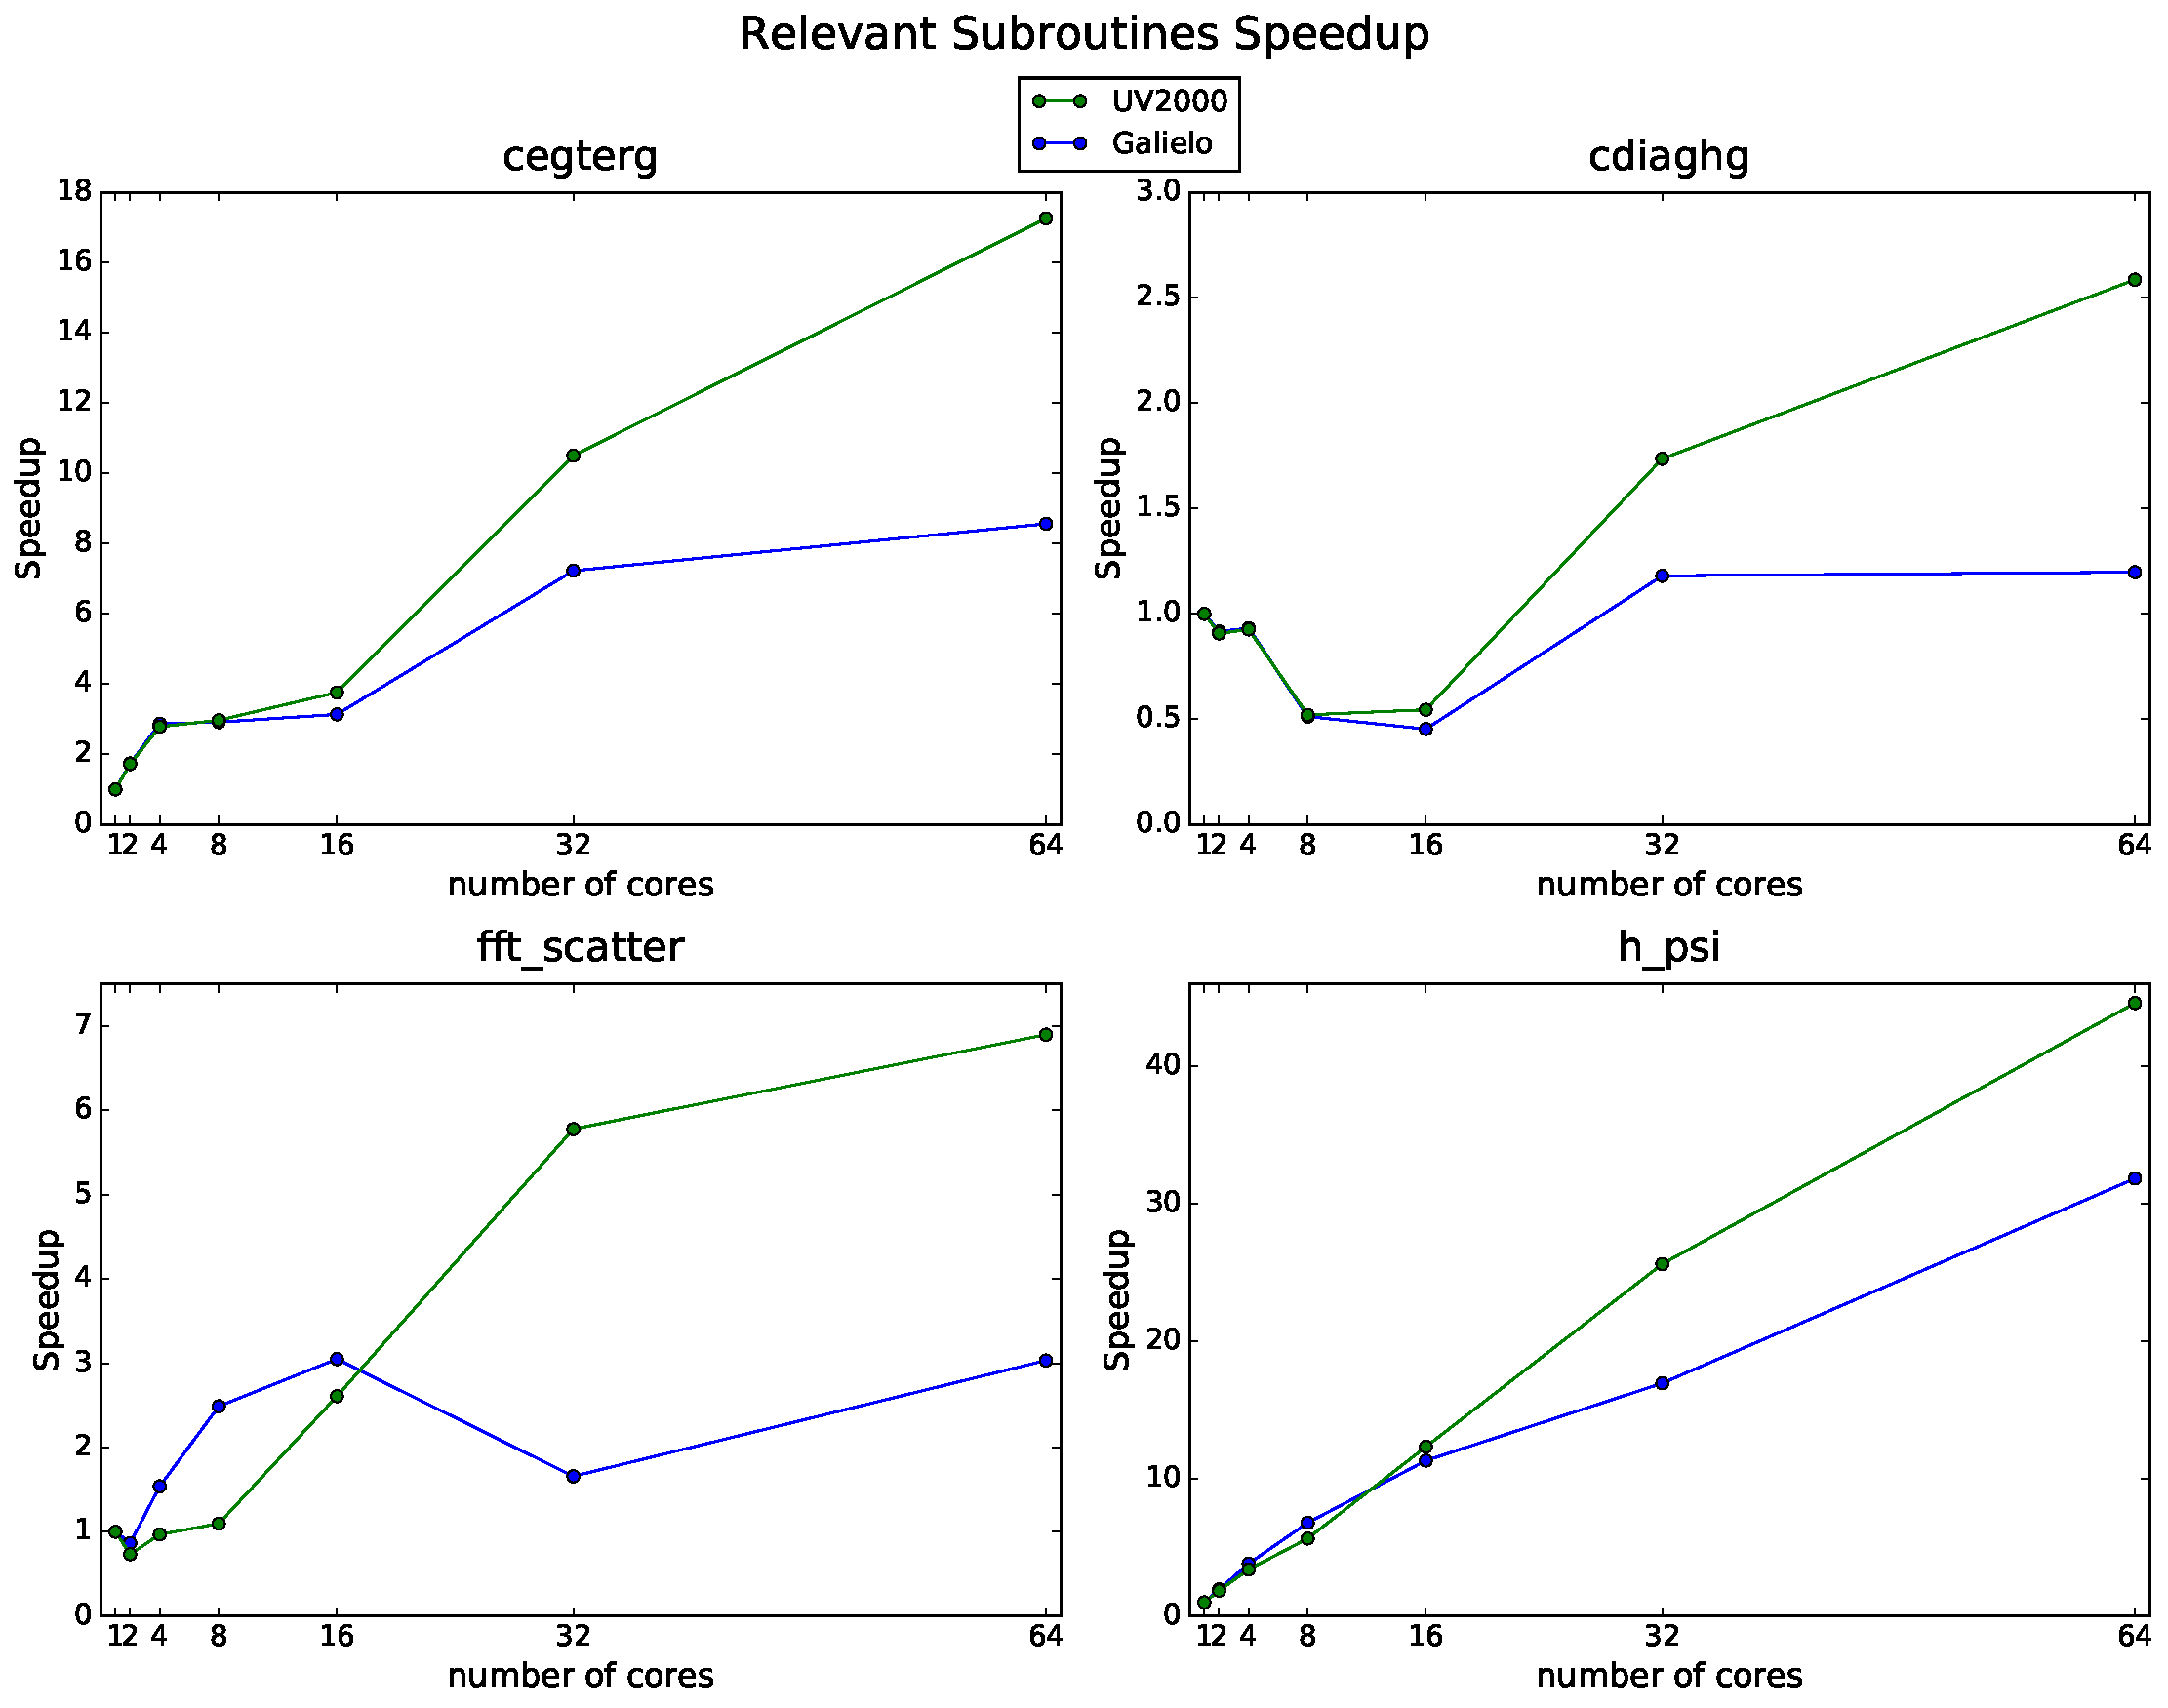
\includegraphics[width=1.1\textwidth]{beam_arch_subroutines.pdf}			
		\end{center}
	\column{0.33\textwidth}
		\begin{overlayarea}{\linewidth}{\textheight}
		\begin{block}{Funzioni}
			\begin{itemize}
				\item<1-> Equazioni di Kohn-Sham
				\item<2-> Diagonalizzazione Hamiltoniana
				\item<3-> Valutazione Hamiltoniana
				\item<4-> Distribuzione griglia
				\item<5-> Comunicazione?
			\end{itemize}		
		\end{block}

		\end{overlayarea}
\end{columns}

\end{frame}

% ********** slide 14 *****************}
\begin{frame}{Dipendenti dall'architettura}
\begin{columns}
	\column{0.6\textwidth}
		\begin{center}			
			\vspace{-1cm}
			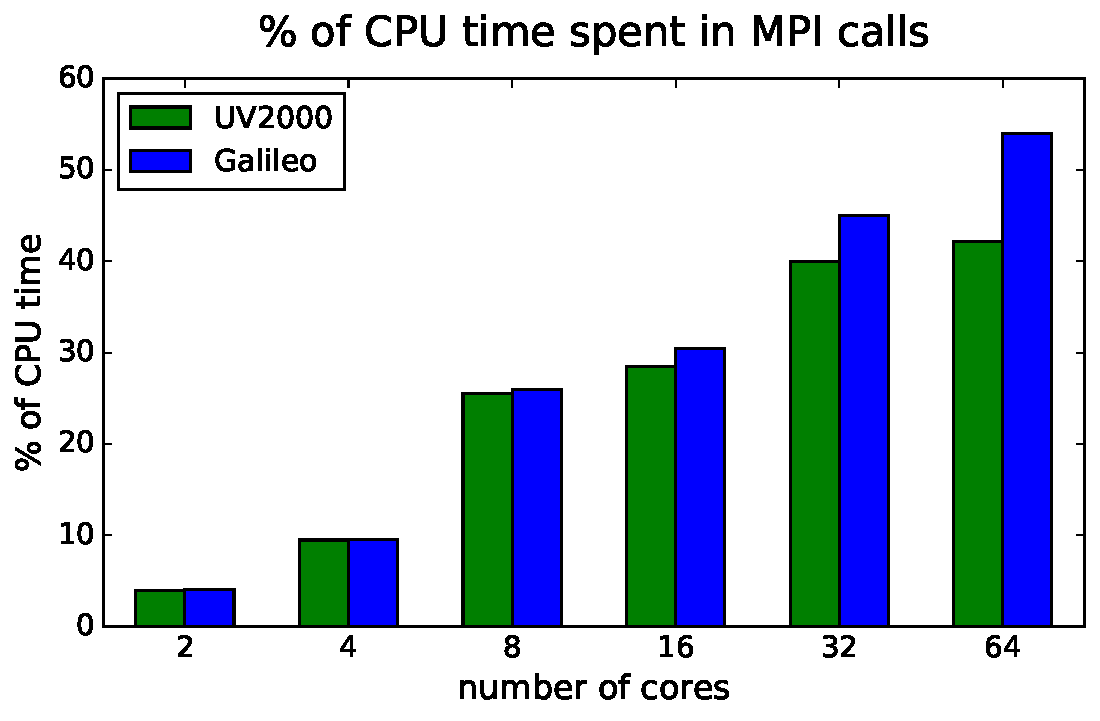
\includegraphics[width=1\textwidth]{arch_mpi_perc.pdf}			
		\end{center}
	\column{0.4\textwidth}
		\begin{overlayarea}{\linewidth}{\textheight}
		\begin{block}{Comunicazione}
			\begin{itemize}
				\item<1-> Ruolo comunicazione cresce sensibilmente
				\item<2-> Oltre il singolo nodo UV200 \`e pi\`u efficiente.
				\item<3-> ScaLAPACK non \`e profilata!
			\end{itemize}		
		\end{block}

		\end{overlayarea}
\end{columns}

\end{frame}



% ********** Conclusioni *****************}

\section{Conclusioni}
\subsection{Conclusioni}

\begin{frame}{Conclusioni}


\end{frame}

\end{document}











\end{document}
